\documentclass[aspectratio=169,xcolor=dvipsnames]{beamer}

% Themes and colors
\usetheme{default}
% \usecolortheme{default}
% \useinnertheme{circles}% http://blogs.ubc.ca/khead/research/research-advice/better-beamer-presentations
\setbeamertemplate{section in toc}[circle]%{3pt}
\setbeamertemplate{navigation symbols}{} % Swith off naviagation symbols: https://nickhigham.wordpress.com/2013/01/18/top-5-beamer-tips/


% Redefine the frametitle template
\makeatletter
\setbeamertemplate{frametitle}{
  \nointerlineskip
  \vspace{0ex}
  \begin{beamercolorbox}[wd=\paperwidth,ht=2.5ex,dp=1ex,left]{frametitle}
    \hspace*{0.4em}\insertframetitle\strut
  \end{beamercolorbox}
}
\makeatother

% Define a custom frame for section opening slides
\newcommand{\sectionframe}[1]{
  \begin{frame}[plain, noframenumbering]
    \vfill % Add vertical space equivalent to the header size
    \centering
    \huge\color{RoyalBlue} #1
    \vfill
  \end{frame}
}

\mode<presentation> {
\setbeamertemplate{caption}[numbered] % https://tex.stackexchange.com/questions/127145/beamer-presentation-figure-has-no-number
\setbeamercolor{background canvas}{bg=white}
\setbeamercolor{title}{fg=RoyalBlue!180}
\setbeamercolor{frametitle}{fg=RoyalBlue!180}
\setbeamercolor{normal text}{fg=black!85}
\setbeamercolor{enumerate item}{bg=RoyalBlue!180}
\setbeamercolor{enumerate subitem}{fg=RoyalBlue!180}
\setbeamercolor{caption name}{fg=RoyalBlue}
\setbeamercolor{itemize item}{fg=RoyalBlue!180}
\setbeamercolor{itemize subitem}{fg=RoyalBlue!180}
\setbeamercolor{section number projected}{bg=Red,fg=white} % https://tex.stackexchange.com/questions/8011/changing-color-and-bullets-in-beamers-table-of-contents
\usepackage{totcount}
\newtotcounter{totalframecount} % Counter for total frame count before appendix
\setbeamertemplate{footline}{
 \hfill \insertframenumber{} / \total{totalframecount}\hspace*{1ex} % \inserttotalframenumber
}
\usepackage[UKenglish]{babel}
% \usepackage[latin1]{inputenc}
\usepackage[T1,OT1]{fontenc}
\usepackage{adjustbox}
\usepackage{graphicx} % Allows including images
\usepackage{apacite} % APA style citations
\usepackage{multirow}
\AtBeginDocument{\urlstyle{APACsame}}  % Links in APA citytions same formatting
\usepackage{natbib} % natbib citations: \citep{} and \citet{} for in-text
% \renewcommand{\bibsection}{\subsubsection*{\bibname } } % https://latex.org/forum/viewtopic.php?t=2701
\def\bibfont{\tiny}
\usepackage{booktabs} % Allows the use of \toprule, \midrule and \bottomrule in tables
% \usepackage{enumitem}
% \setitemize{label=\textbullet, font=\large \color{Red}, itemsep=12pt} %  %https://stackoverflow.com/questions/4968557/latex-very-compact-itemize
% https://tex.stackexchange.com/questions/16793/global-setting-of-spacing-between-items-in-itemize-environment-for-beamer
\let\OLDitemize\itemize
\renewcommand\itemize{\OLDitemize\addtolength{\itemsep}{10pt}}
\let\OLDenumerate\enumerate
\renewcommand\enumerate{\OLDenumerate\addtolength{\itemsep}{10pt}}
\usepackage{amsmath}
\usepackage{float}

\usepackage{hyperref}
\hypersetup{
    colorlinks=true,
    linkcolor=MidnightBlue,
    urlcolor=MidnightBlue, %teal,
    citecolor=MidnightBlue
}

% \graphicspath{{./figures/}} %this is the file in which you should save figures
}

% Title page information
\title{Optimal Road Investments in CEMAC}
% \subtitle{Your Presentation Subtitle}
\author{Sebastian Krantz}
\institute{Kiel Institute for the World Economy\\ RC International Development}
\date{\today} 

\begin{document}

\begin{frame}[plain, noframenumbering]
\titlepage 
\end{frame}

%----------------------------------------------------------------------------------------
%	PRESENTATION SLIDES
%----------------------------------------------------------------------------------------

\begin{frame}[plain, noframenumbering]
\frametitle{Outline}
\tableofcontents
\end{frame}

%------------------------------------------------
\section{Introduction}
%------------------------------------------------

\begin{frame}{Introduction} \vspace{-1mm}
CEMAC region (CMR, CAF, TCD, COG, GNQ, GAB) has slow network, high border costs, and low share of intra-regional exports (8\% vs. 19.3\% WAEMU) vs. Africa. \\ \vspace{2mm}
\resizebox{\textwidth}{!}{
\begin{tabular}{cc}
\includegraphics[width=0.5\textwidth, trim= {3mm 0 3mm 0}, clip]{"/Users/sebastiankrantz/Documents/IFW Kiel/Africa-Infrastructure/quantitative_model_paper/figures/network_time_efficiency_new.pdf"} & 
\includegraphics[width=0.47\textwidth, trim= {1cm 0 1cm 0.4cm}, clip]{"/Users/sebastiankrantz/Documents/IFW Kiel/Africa-Infrastructure/quantitative_model_paper/figures/DBS_border_dist_km_adj_map.pdf"} 
\end{tabular}
}
\end{frame}

\begin{frame}{Introduction}
Roads account for 80-90\% of passenger and freight traffic, but low network density (50km/1000$km^2$), $\sim$85\% in poor condition, and $<$50\% of rural pop. live near an all-\\season road. $\Rightarrow$ World Bank has $\sim$2 billion USD of transport projects in the region. \\ \vspace{2mm}    
\resizebox{\textwidth}{!}{
\begin{tabular}{@{}c@{}c@{}}
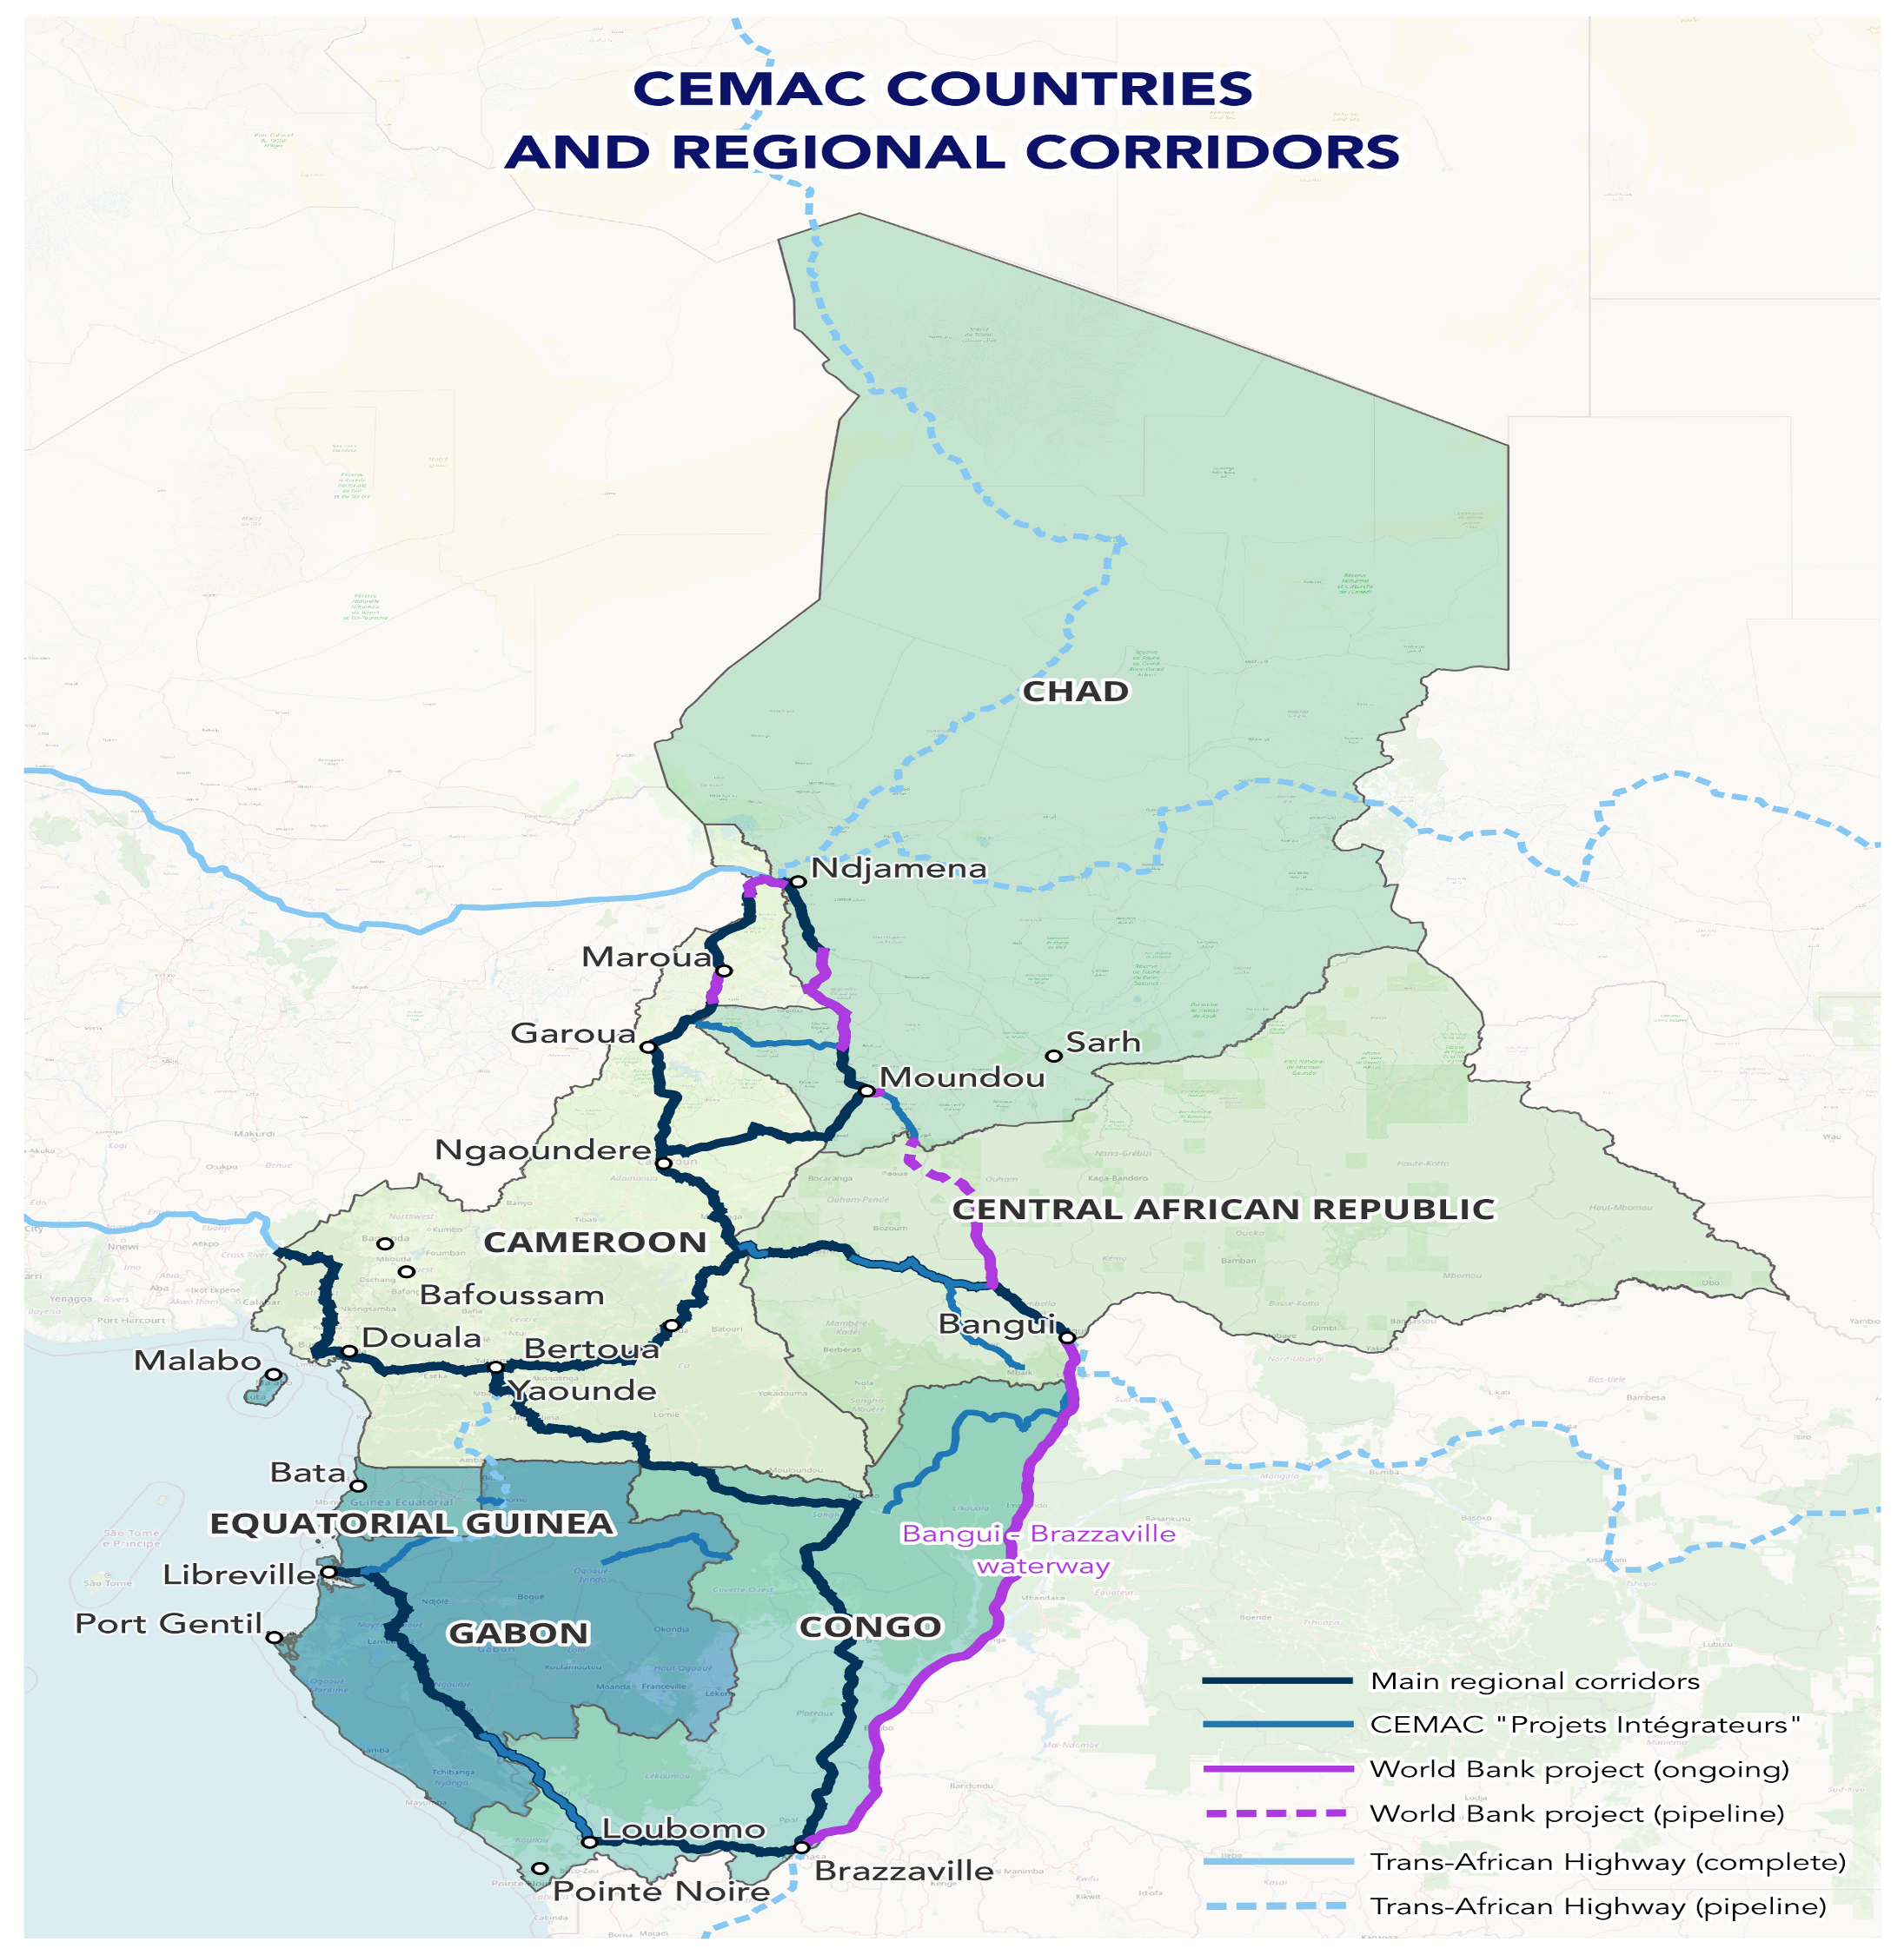
\includegraphics[width=0.58\textwidth, trim= {5mm 0 2mm 5.1cm}, clip]{"../figures/CEMAC_Projects.png"} & 
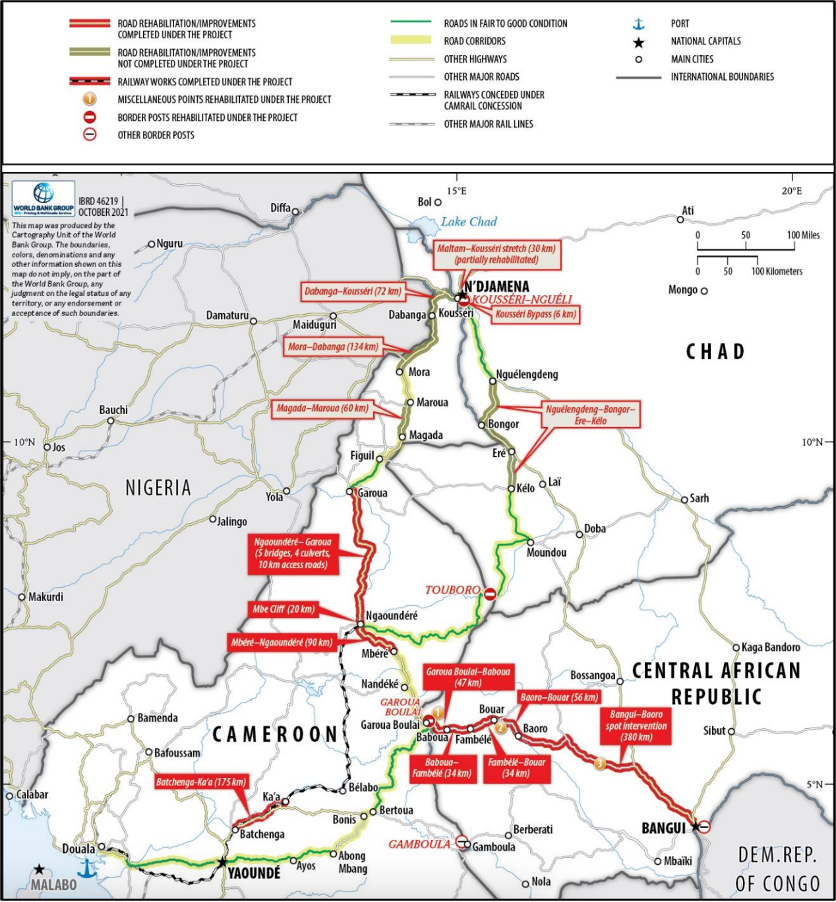
\includegraphics[width=0.42\textwidth, trim= {0 0 0 0}, clip]{"../figures/CEMAC_Projects_WB.png"} 
\end{tabular}
}
\end{frame}

\begin{frame}{This Paper/Project}
Characterizes \textbf{economically optimal} regional road network investments in \textbf{partial and general equilibrium} (market access and welfare maximization) taking into account: \\ \vspace{5mm}
\begin{itemize}
\item Detailed road network data and quality estimates (Google Maps travel speed)
\item Detailed wealth, agricultural production, and population data $\to$ high-resolution market access/productivity measures
\item Heterogeneous road construction/upgrading costs (a function of road quality, terrain ruggedness, population density, and local conflict intensity/security)
\item Border frictions and trade through international ports $\to$ additional assessment of optimal investments in border posts along border-crossing links
\item Several planning budgets and objectives (with/without inequality aversion)
\end{itemize}
\end{frame}

%------------------------------------------------
\section{Data}
%------------------------------------------------

\sectionframe{Data}

\begin{frame}{Road Network} \vspace{-3mm}
\begin{adjustbox}{center}
    \begin{columns} \setlength{\columnsep}{1mm} % Set the space between columns to 1 cm
        % Left column
        \begin{column}{0.22\textwidth}
\small 54 largest cities with radius $>$100km, incl. 6 intnl. ports $\to$\\\vspace{2mm} connected with 1431 fastest car routes (OpenStreetMap $+$ Graphhopper) $\to$\\\vspace{2mm} network with 196 nodes and 313 edges $+$ 71 additional links with $>50$\% route efficiency gains (27.1\% longer than GCD: link mean) $\to$\\\vspace{2mm} parameterized with Google Maps speed (new links 0 speed).
        \end{column}
        % Right column
        \begin{column}{0.9\textwidth}
\resizebox{\textwidth}{!}{
\begin{tabular}{@{}c@{}c@{}}
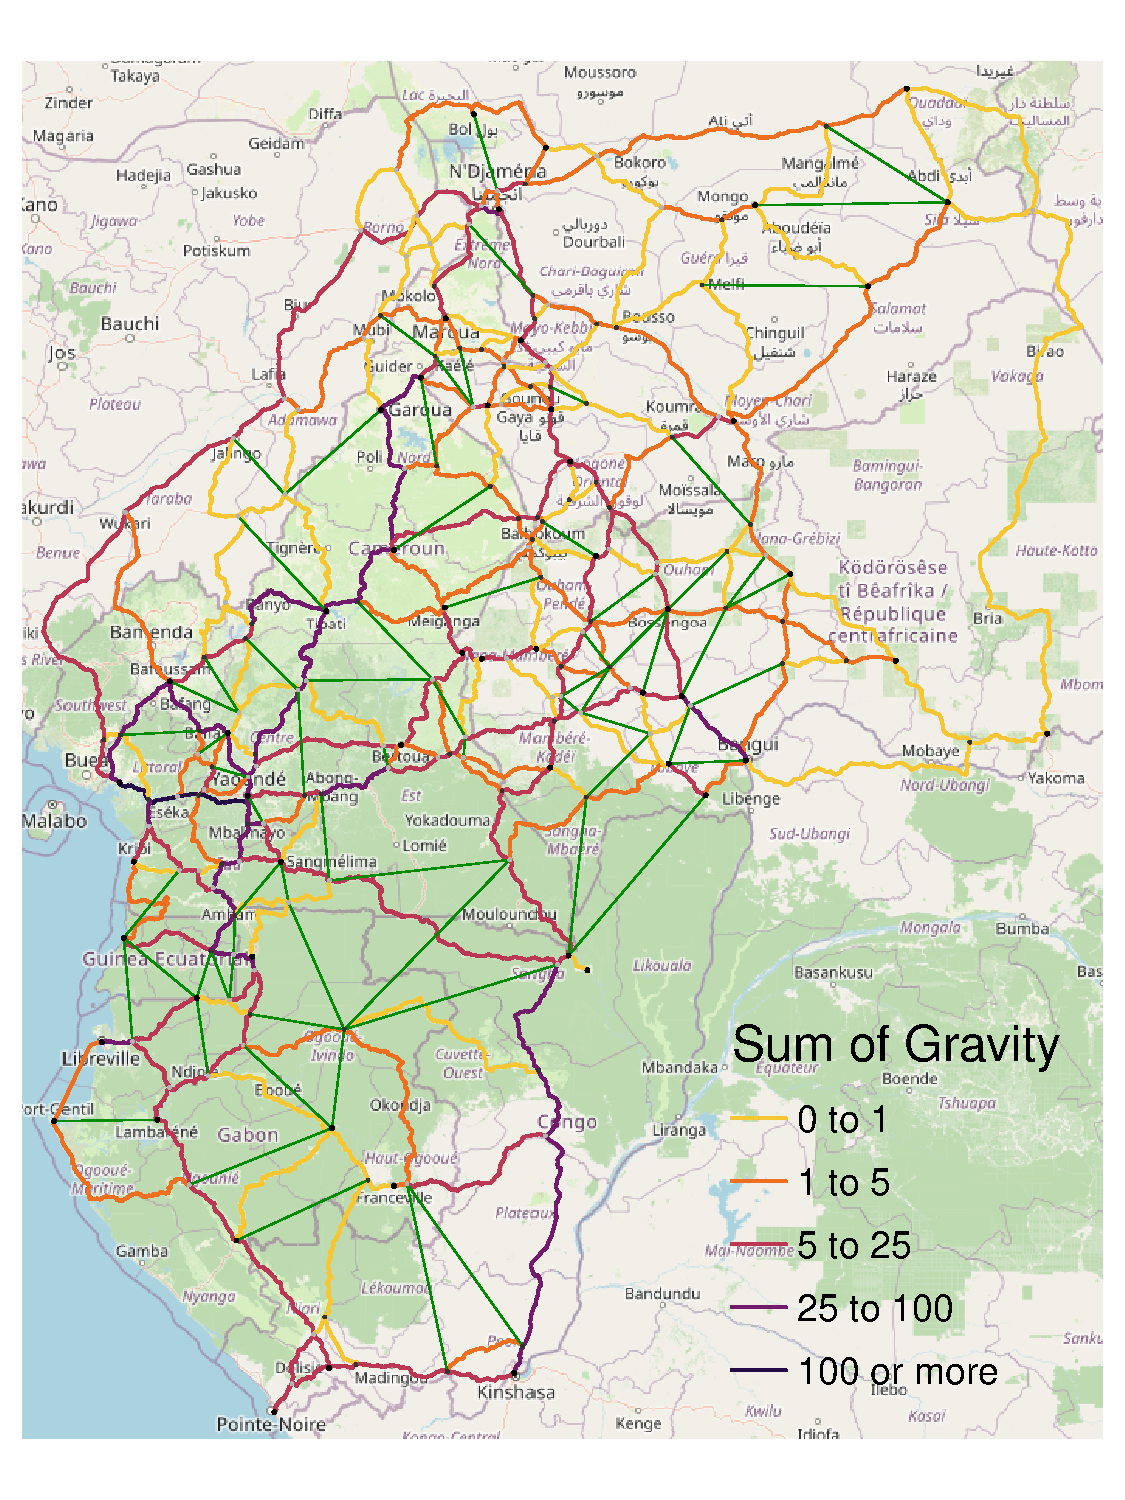
\includegraphics[width=0.5\textwidth]{"../figures/trans_CEMAC_network_actual_discretized_gravity_new_roads_real_edges.pdf"} & 
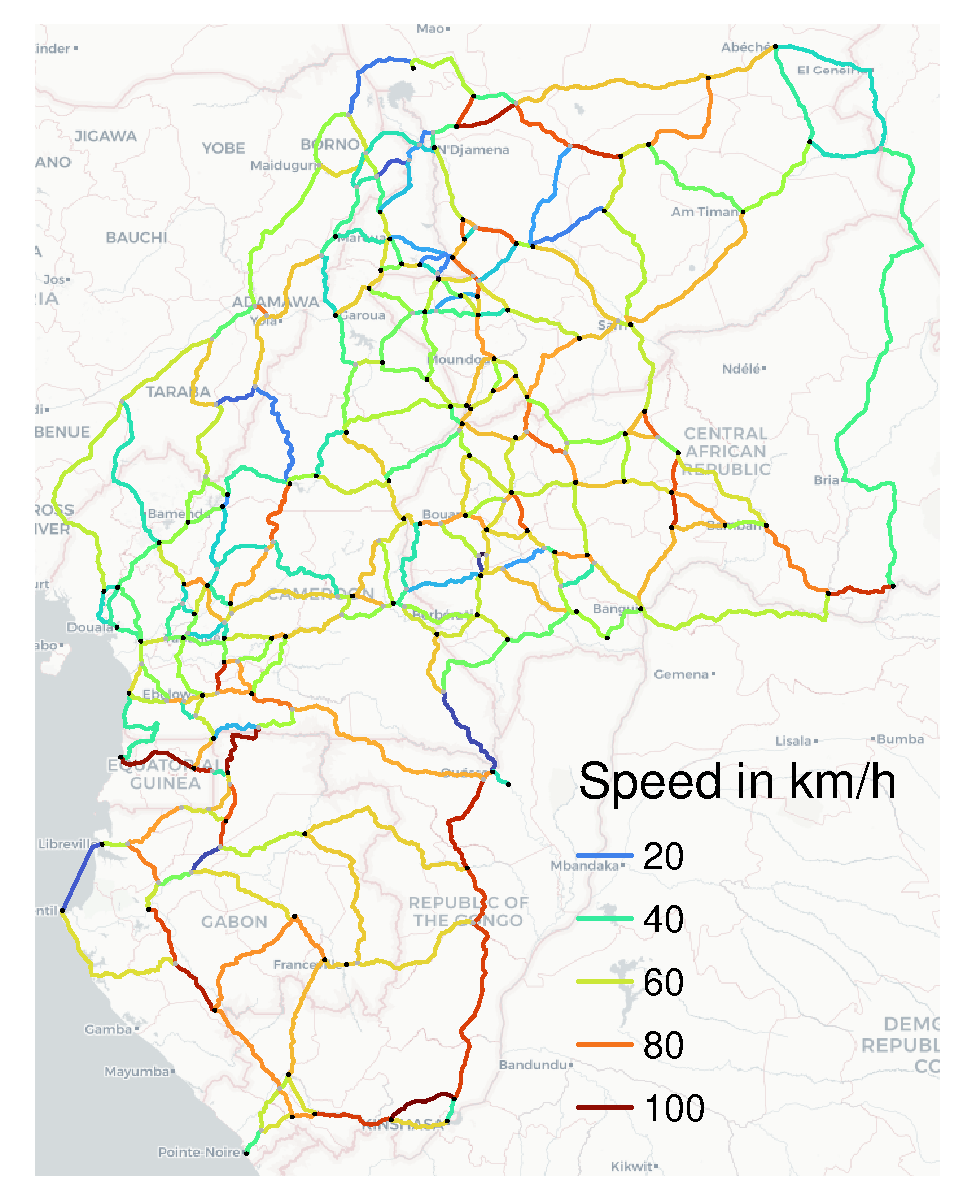
\includegraphics[width=0.5\textwidth, trim= {2mm 0 7mm 2mm}, clip]{"../figures/trans_CEMAC_network_average_link_speed_google.pdf"}
\end{tabular}
}
        \end{column}
    \end{columns}
  \end{adjustbox}
\end{frame}


\begin{frame}{Household Wealth and Agricultural Production} \vspace{-3mm}
\begin{adjustbox}{center}
    \begin{columns} \setlength{\columnsep}{1mm} % Set the space between columns to 1 cm
        % Left column
        \begin{column}{0.23\textwidth}
  
\small High-resolution International Wealth Index \citep{lee2022high} and total crop production \citep{SPAM} of region's 11 most important crops accounting for 80\% of total production:\\\vspace{3mm}
\scriptsize
CASS (19.8), PLNT (13), OILP (6.7), SUGC (6.7), MAIZ (6.6), ORTS (5.5), SORG (5.4), VEGE (4.5), YAMS (4.4), GROU (3.8), BANA (3.5).
        \end{column}
        % Right column
        \begin{column}{0.85\textwidth}
\resizebox{\textwidth}{!}{
\begin{tabular}{@{}c@{}c@{}}
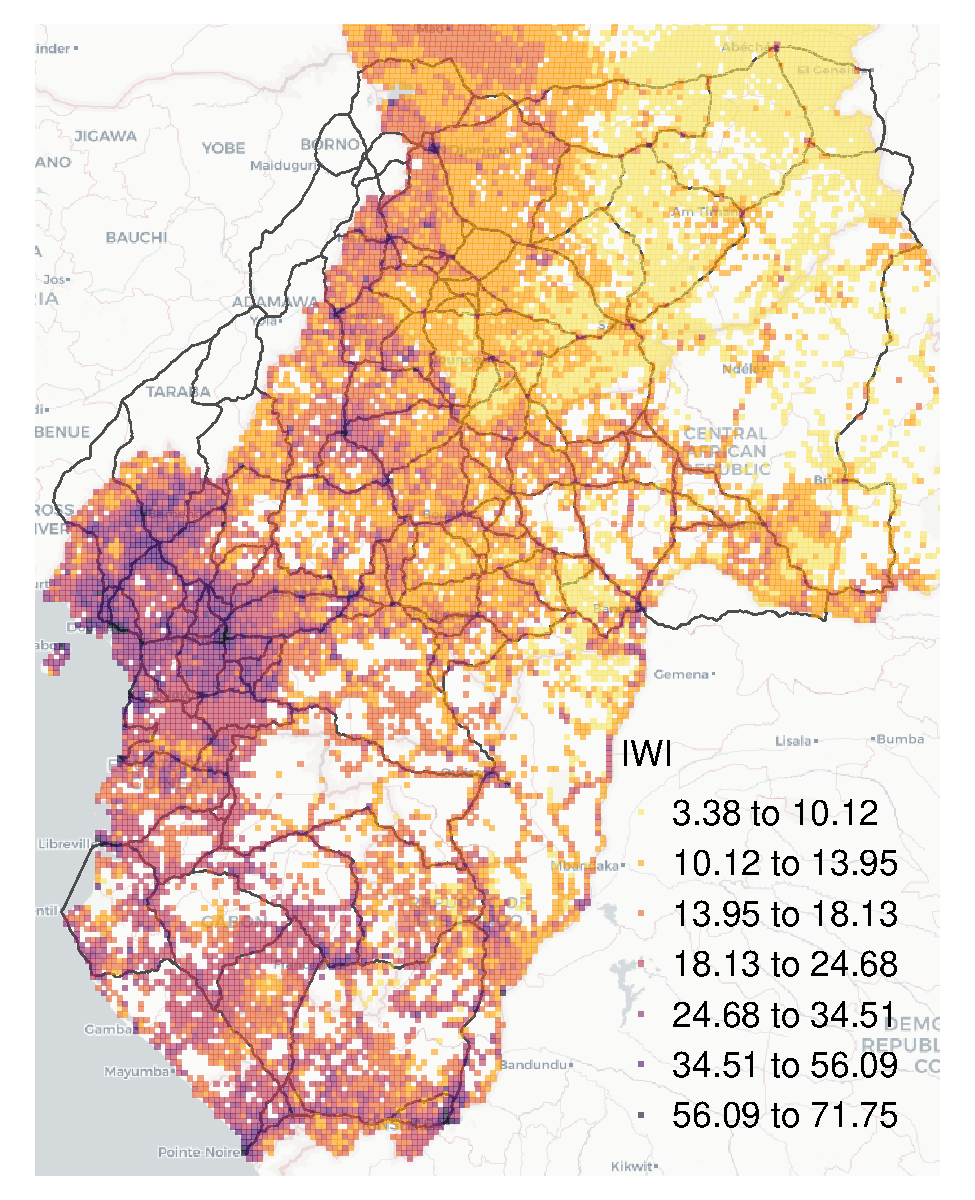
\includegraphics[width=0.5\textwidth, trim= {5mm 0 5mm 0}, clip]{"../figures/IWI_CEMAC_GRID.pdf"} & 
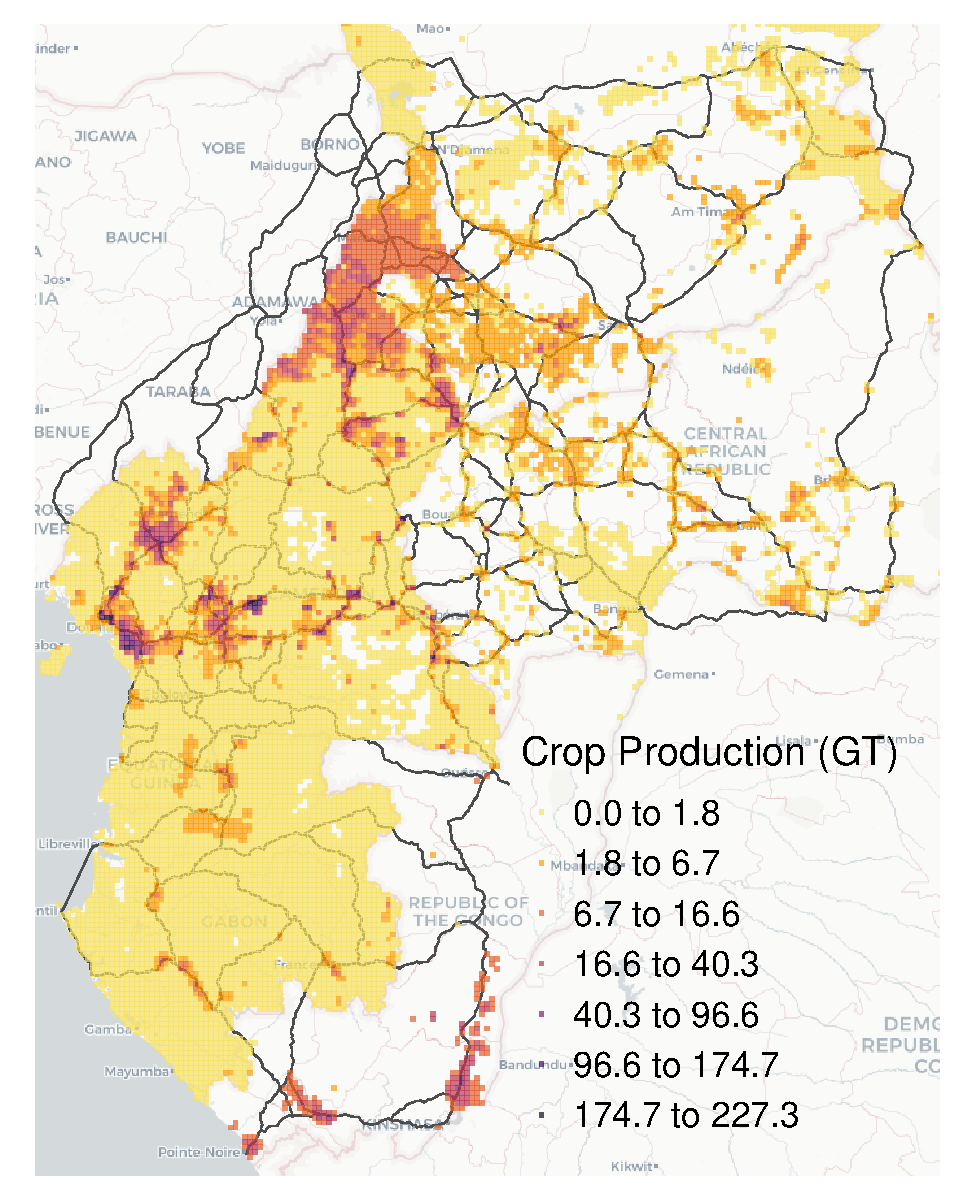
\includegraphics[width=0.5\textwidth, trim= {5mm 0 5mm 0}, clip]{"../figures/crops/SPAM_CEMAC_TOP80.pdf"}
\end{tabular}
}
        \end{column}
    \end{columns}
  \end{adjustbox}
\end{frame}

\begin{frame}{Total Production} \vspace{-3mm}
\small Multiply IWI with Africapolis 2025 populations within 30km of each node and scale to 80\% of CEMAC 2023 GDP (90.9 billion 2015 USD). CROP production (within 50km of each node) is 20\% of GDP (GDP weighted average of AFF sectors is 15\% and population weighted is 25\%). 
\begin{adjustbox}{center}
\begin{tabular}{@{}c@{}c@{}@{}c@{}}
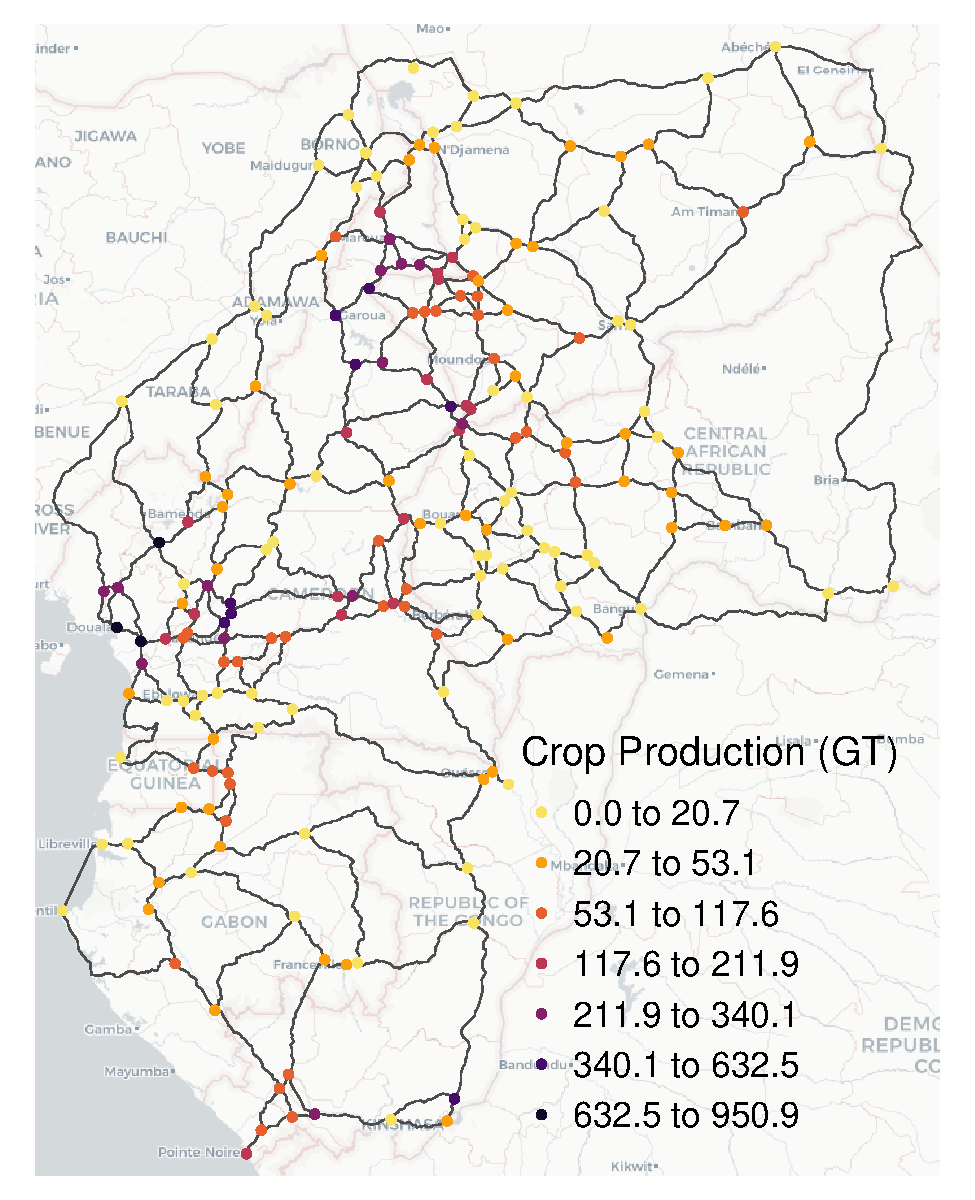
\includegraphics[width=0.38\textwidth, trim= {7mm 0 7mm 0}, clip]{"../figures/trans_CEMAC_network_SPAM_TOP80.pdf"} & 
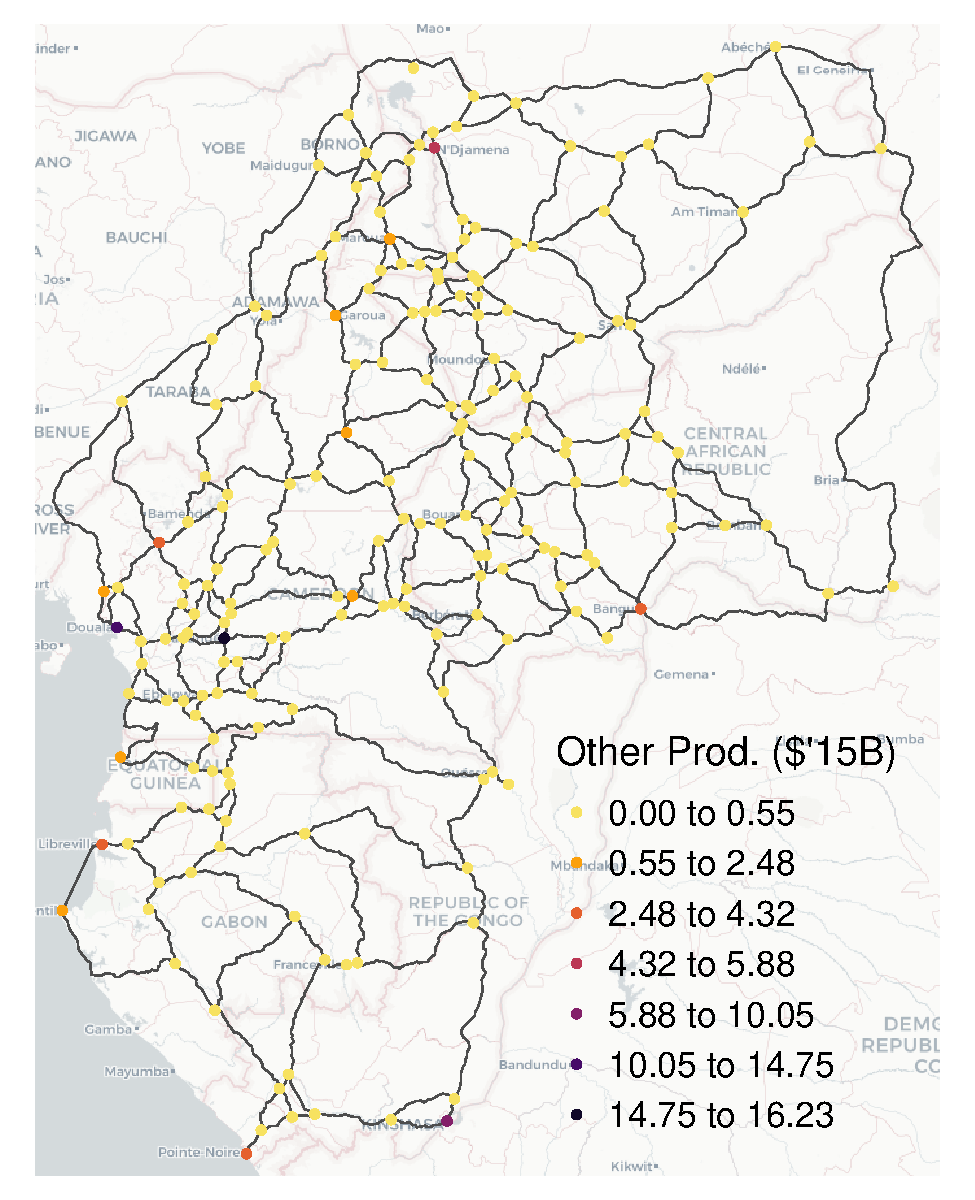
\includegraphics[width=0.38\textwidth, trim= {7mm 0 7mm 0}, clip]{"../figures/trans_CEMAC_network_GDP_other.pdf"} & 
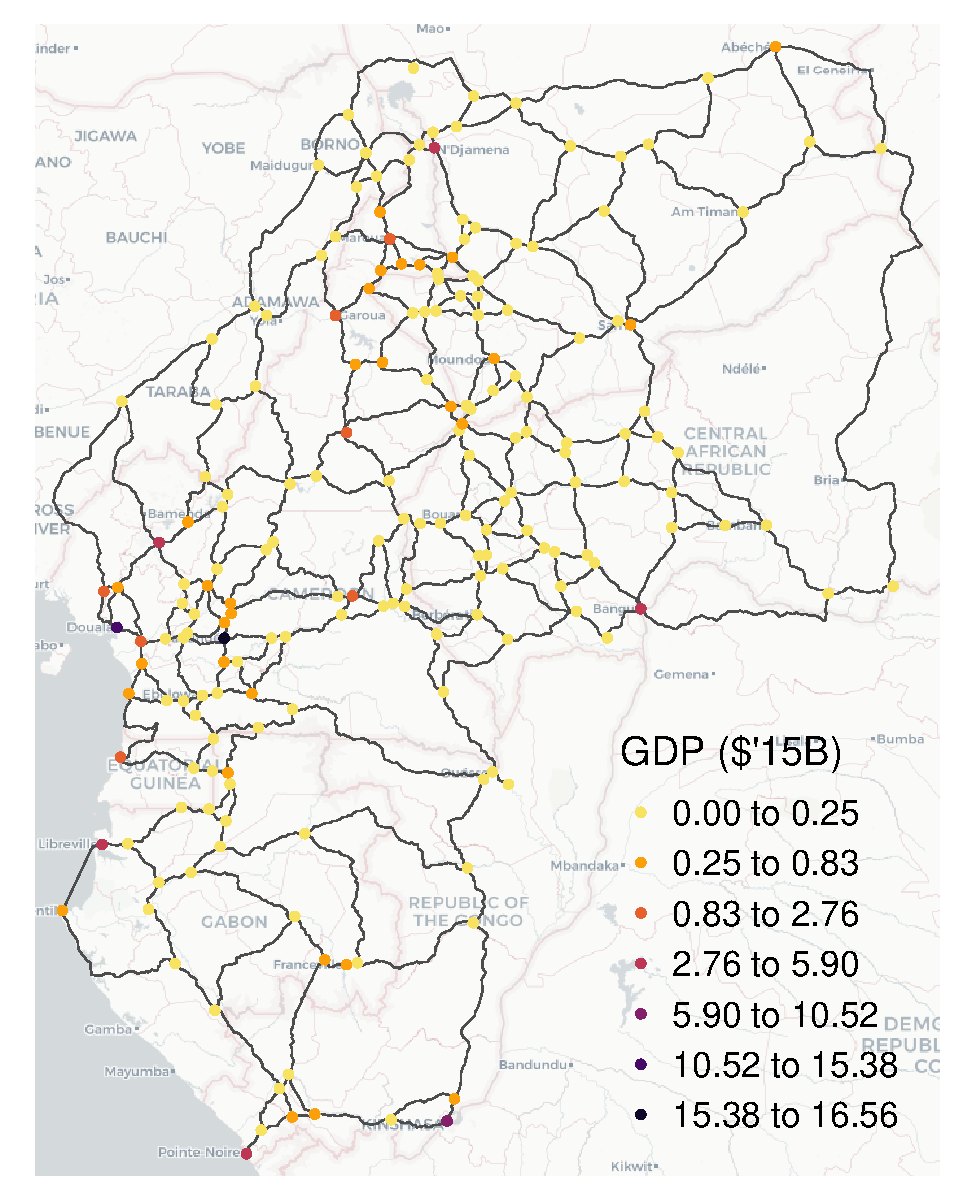
\includegraphics[width=0.38\textwidth, trim= {7mm 0 7mm 0}, clip]{"../figures/trans_CEMAC_network_GDP.pdf"}
\end{tabular}
  \end{adjustbox}
\end{frame}


\begin{frame}{Border Frictions: Doing Business Surveys} \vspace{-3mm}
\small 2019 border compliance time of trading standardized product $+$ time/cost converted to road time/distance as in \citet{krantz2024optimal}: dividing cost by 1.6 and documentary/border time by 10/4.
\begin{adjustbox}{center}
\begin{tabular}{@{}c@{}c@{}@{}c@{}}
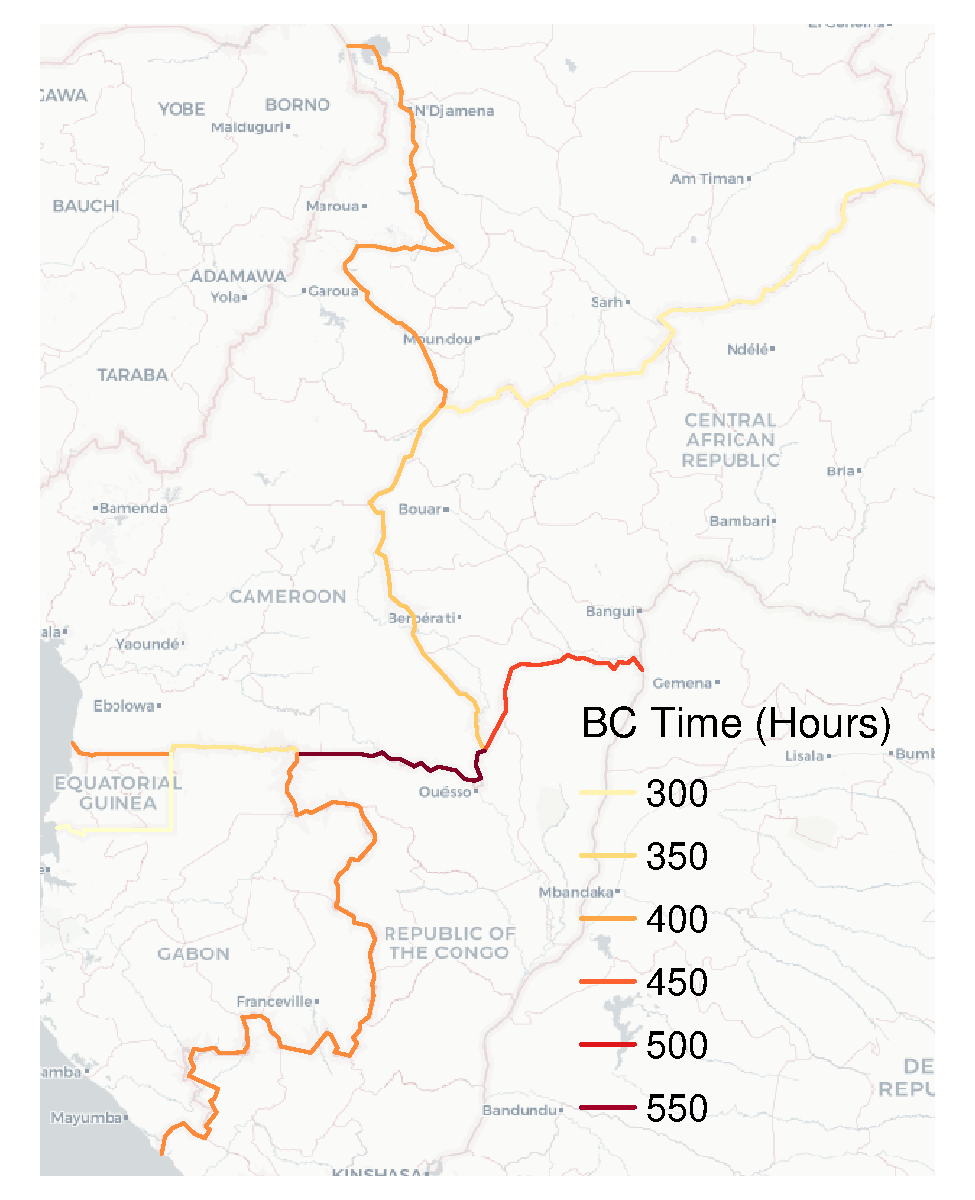
\includegraphics[width=0.38\textwidth, trim= {1cm 0 1cm 0}, clip]{"../figures/trade_costs/DBS_border_time_hours_map.pdf"} & 
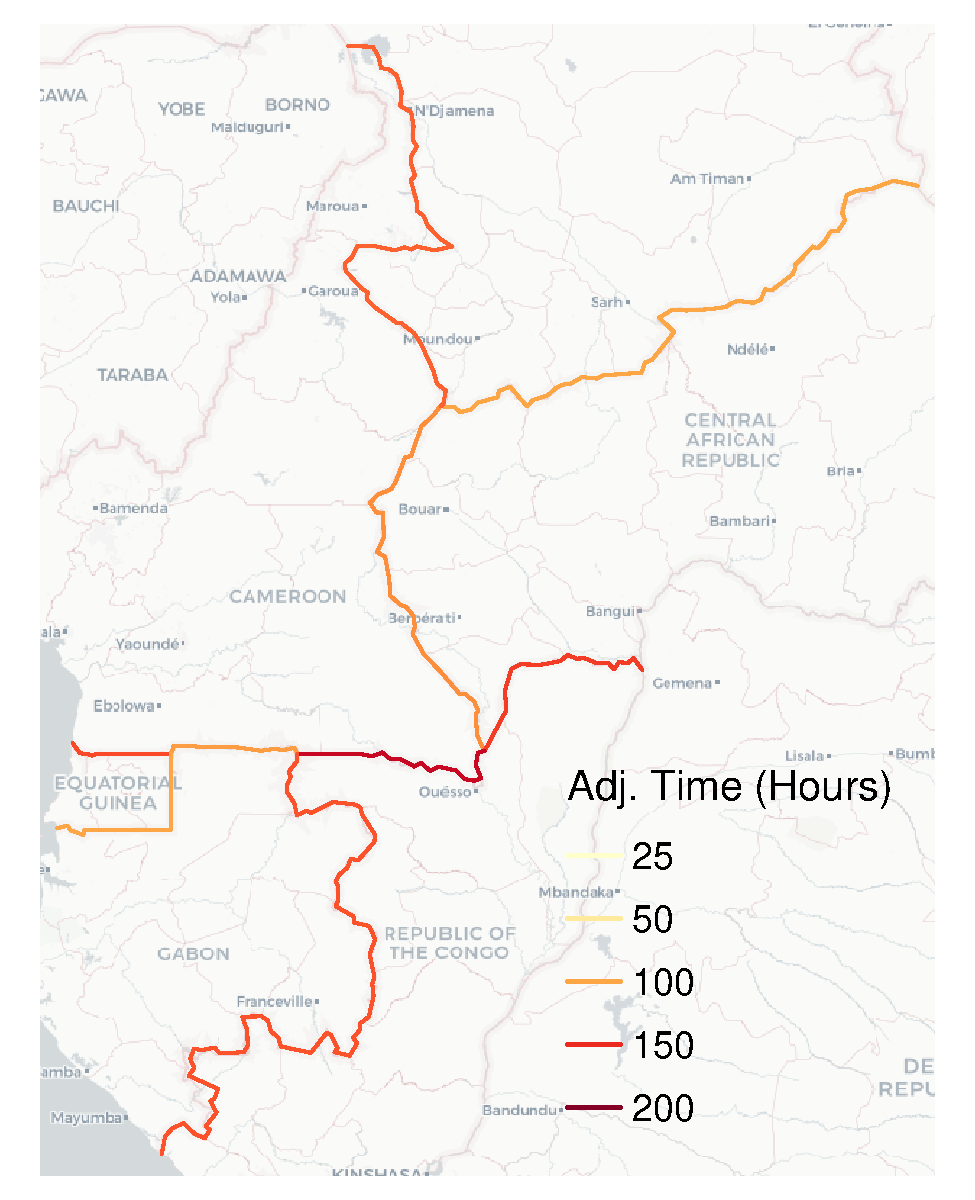
\includegraphics[width=0.38\textwidth, trim= {1cm 0 1cm 0}, clip]{"../figures/trade_costs/DBS_border_time_hours_adj_map.pdf"} & 
\includegraphics[width=0.38\textwidth, trim= {1cm 0 1cm 0}, clip]{"../figures/trade_costs/DBS_border_dist_km_adj_map.pdf"}
\end{tabular}
\end{adjustbox}
\end{frame}

\begin{frame}{Road Construction/Upgrading Costs $\sim$ Following \citet{collier2016cost}} 
\small $\ln\left(\frac{\text{cost}}{km}\right) = \ln(X) -0.11 \times (\text{len} > 50km) + 0.12 \times \ln(\text{rugg}) + 0.085 \times \ln(\frac{\text{pop}}{km^2}) + 0.1 \times \ln(\sum\sqrt{\text{fat}})$ 
\begin{adjustbox}{center}
\begin{tabular}{@{}c@{}c@{}@{}c@{}}
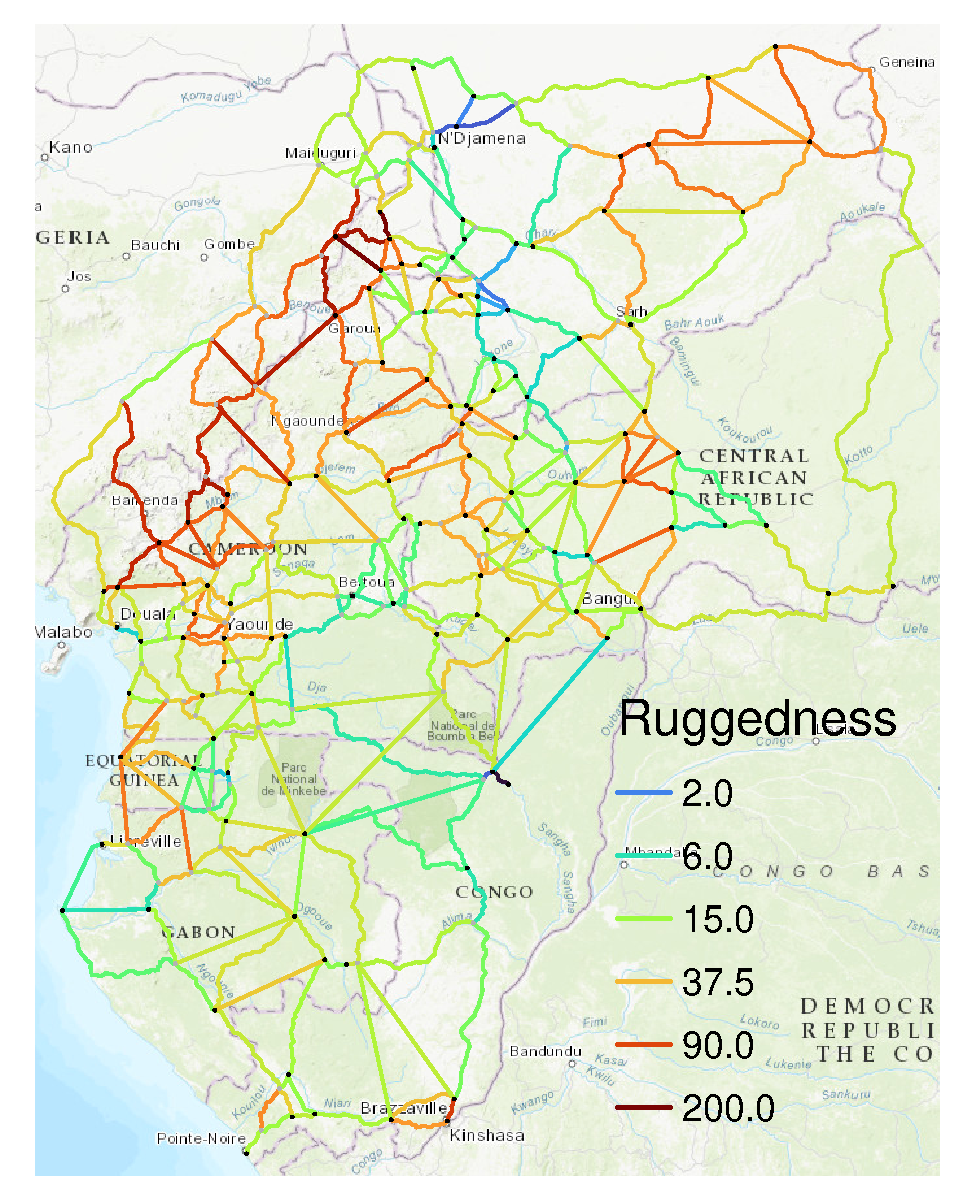
\includegraphics[width=0.38\textwidth, trim= {1cm 0 1cm 0}, clip]{"../figures/trans_CEMAC_network_rugg.pdf"} & 
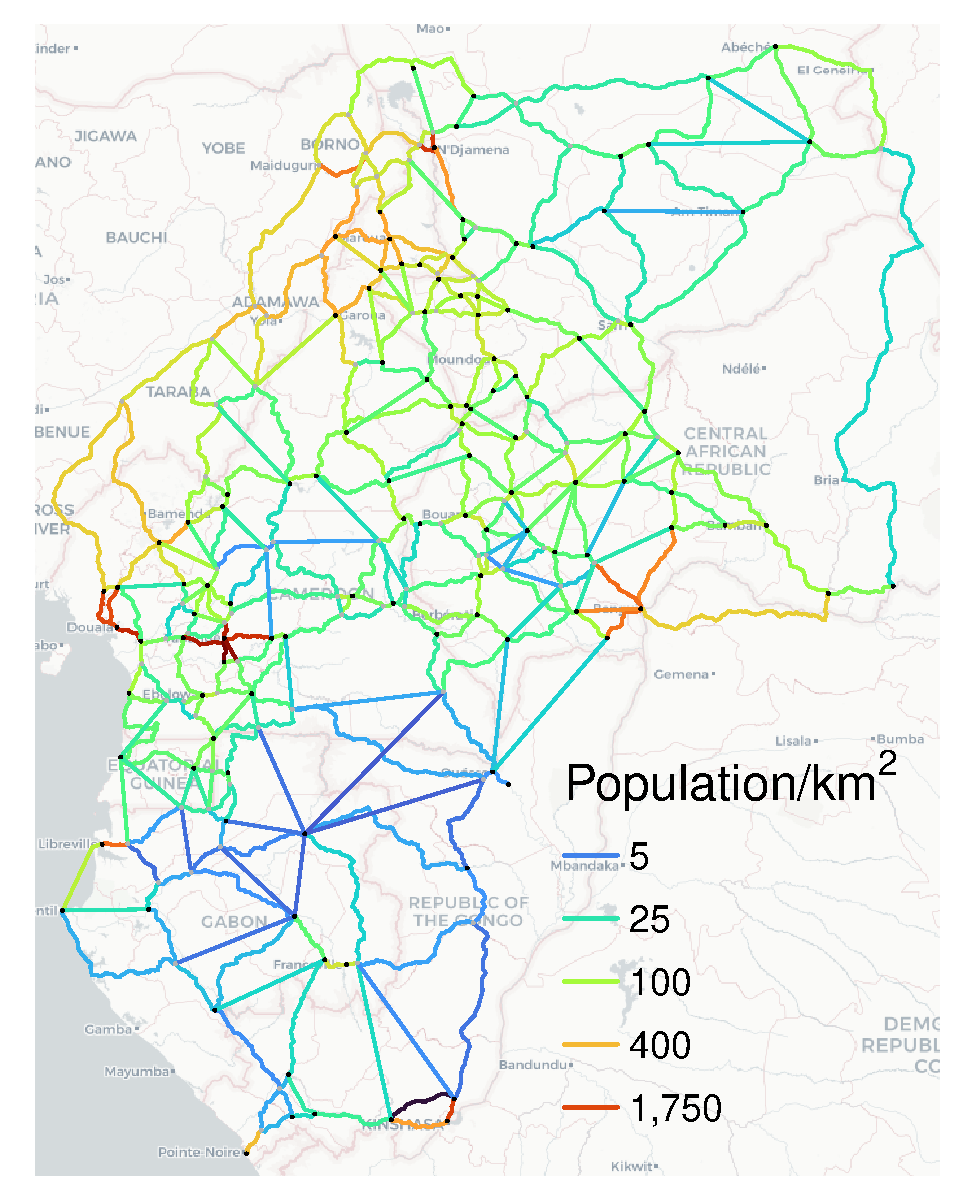
\includegraphics[width=0.38\textwidth, trim= {1cm 0 1cm 0}, clip]{"../figures/trans_CEMAC_network_pop_wpop_km2.pdf"} & 
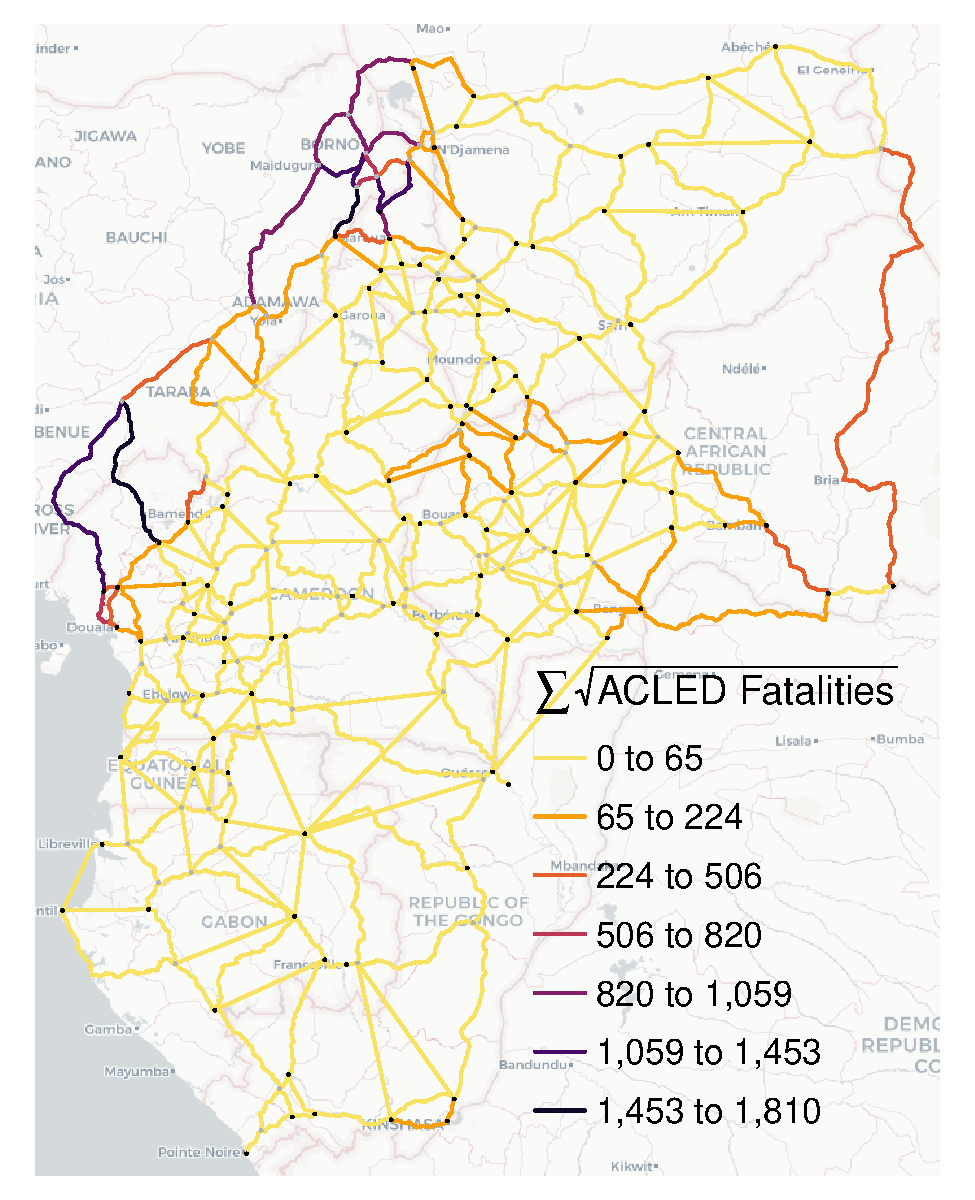
\includegraphics[width=0.38\textwidth, trim= {1cm 0 1cm 0}, clip]{"../figures/trans_CEMAC_network_ACLED_edges_add.pdf"}
\end{tabular}
\end{adjustbox}
\end{frame}

\begin{frame}{Road Construction/Upgrading Costs $\sim$ Following \citet{collier2016cost}} \vspace{-2mm}
\small World Bank ROCKS 2018: 
2L highway in Africa costs \textbf{611K} USD'15/km $\Rightarrow$ $X$ = 120K for new roads, $X$ = 101.6K for upgrades, $X$ = 64.6K for mixed works, and $X$ = 28.4K for resurfacing.
\begin{adjustbox}{center}
\begin{tabular}{@{}c@{}c@{}@{}c@{}} 
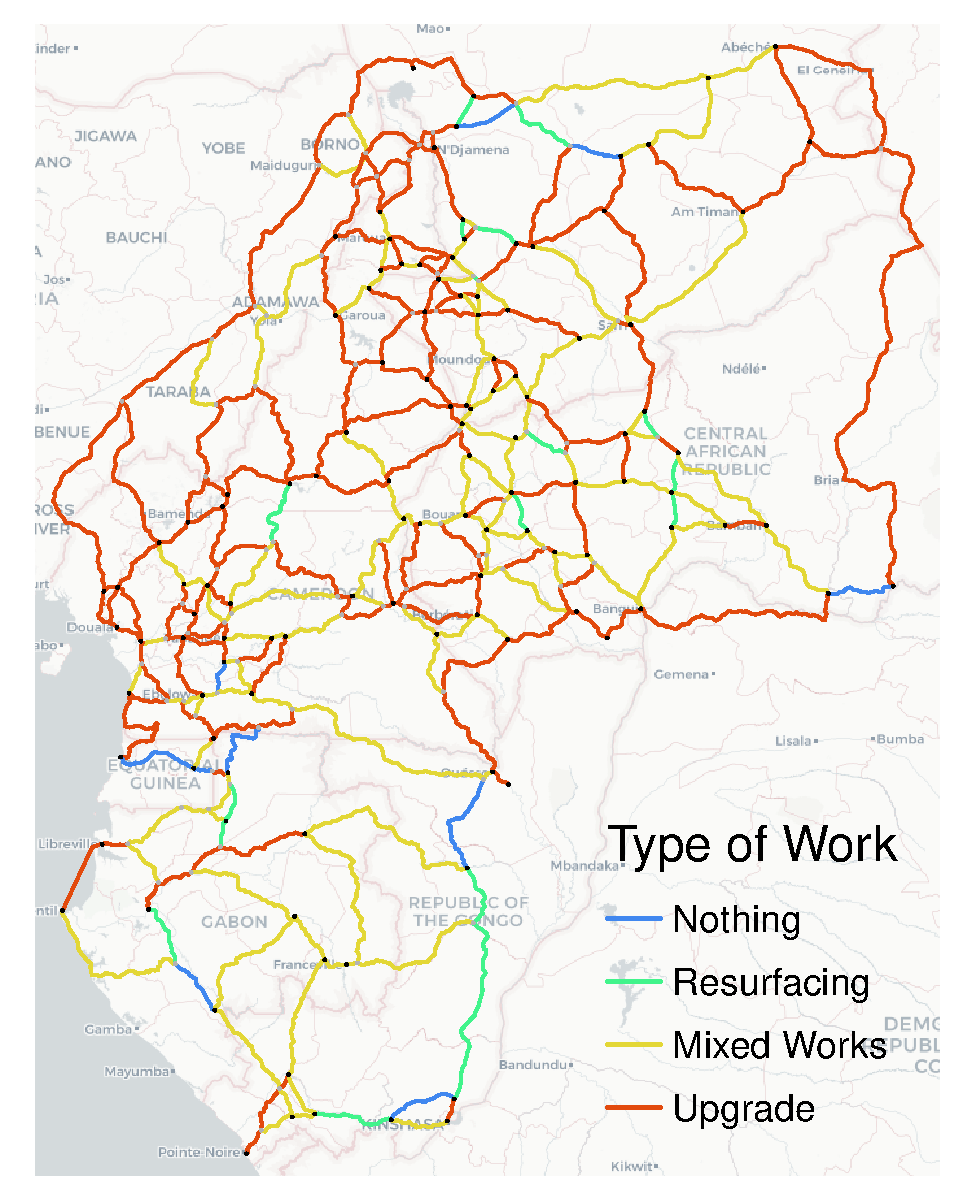
\includegraphics[width=0.38\textwidth, trim= {0.9cm 0 0.9cm 0}, clip]{"../figures/trans_CEMAC_network_type_of_work_google.pdf"} & 
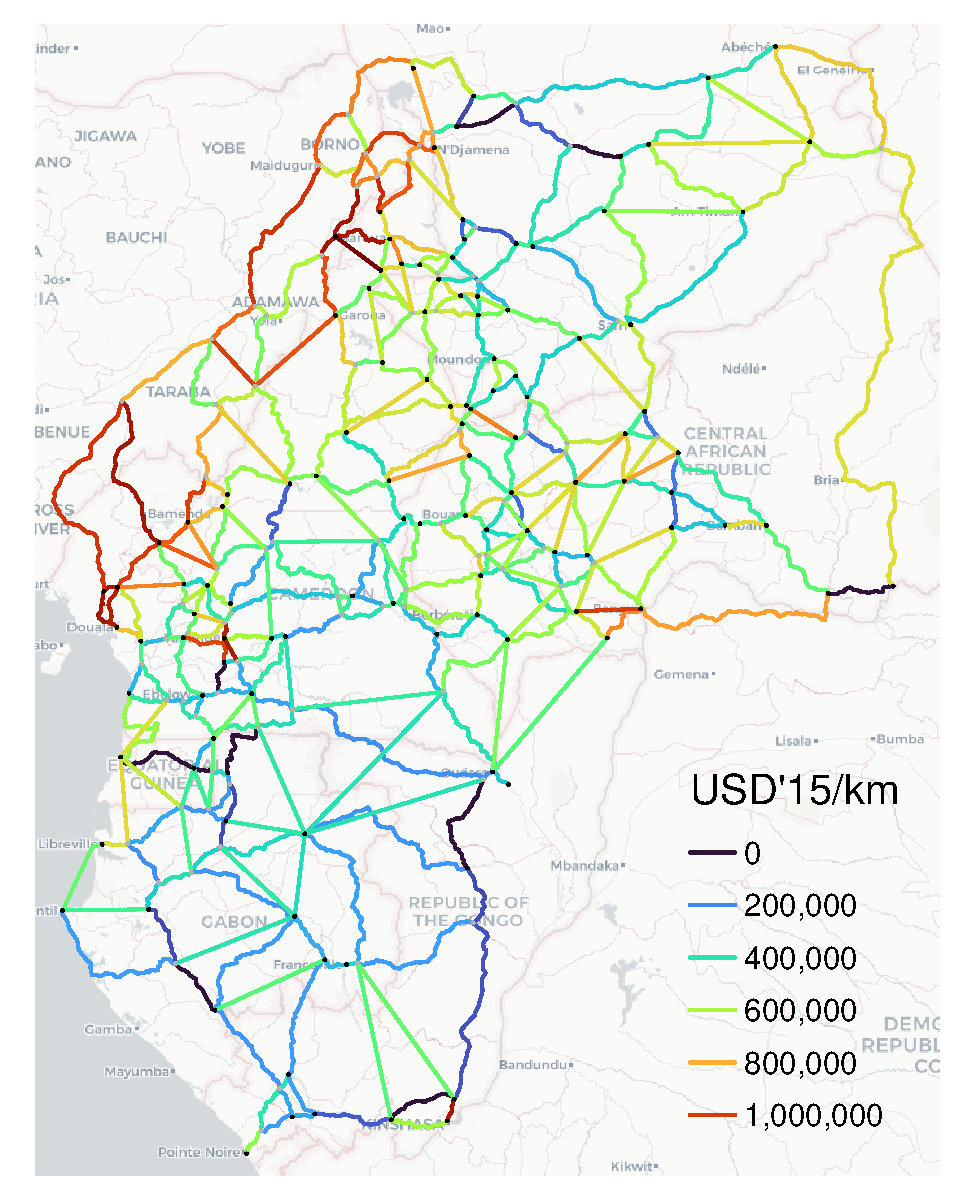
\includegraphics[width=0.38\textwidth, trim= {0.9cm 0 0.9cm 0}, clip]{"../figures/trans_CEMAC_network_all_costs_conflict_google.pdf"} & 
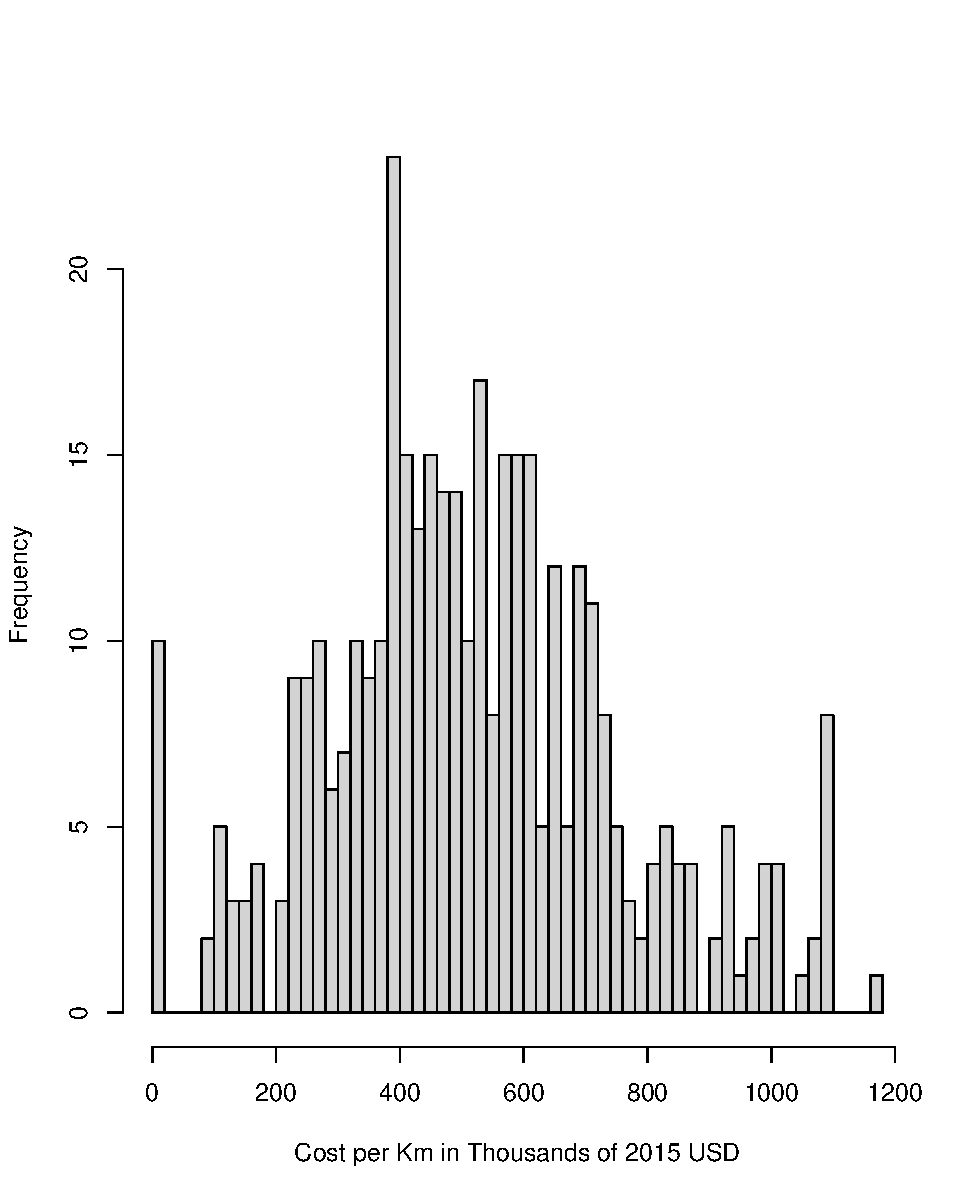
\includegraphics[width=0.38\textwidth, trim= {0.5cm 0 0.5cm 2cm}, clip]{"../figures/trans_CEMAC_network_all_costs_conflict_hist_google.pdf"} 
\end{tabular}
\end{adjustbox}
\end{frame}


%------------------------------------------------
\section{Optimal Investments in Partial Equilibrium}
%------------------------------------------------

\sectionframe{Optimal Investments in Partial Equilibrium}

\begin{frame}{Upgrading Network to 90km/h - MA (GDP/Minute) Gains}
\vspace{-2mm}
Upgrading links to $\geq$90km/h (p97) costs \$19B and yields \textbf{63.8\%} MA gain (LHS, 0.85\$/min/\$), and \textbf{60.2\%} (0.47\$/min/\$) under frictions. Median ratio: 0.42 ($\downarrow$58\%).
\begin{adjustbox}{center}
\begin{tabular}{@{}c@{}c@{}@{}c@{}} 
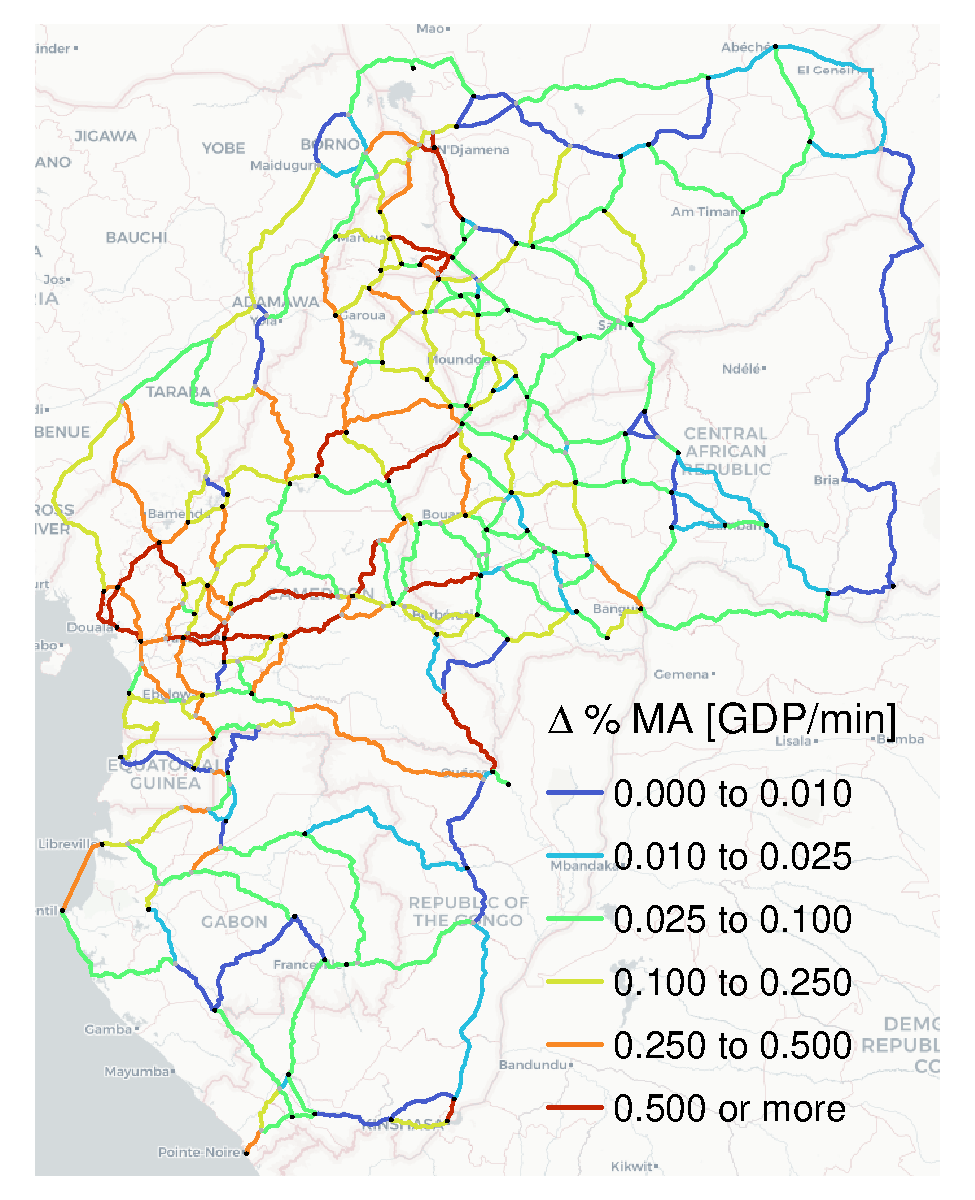
\includegraphics[width=0.38\textwidth, trim= {0.9cm 0 0.9cm 0}, clip]{"../figures/PE/trans_CEMAC_network_MACR_90_min_speed_perc_google.pdf"} & 
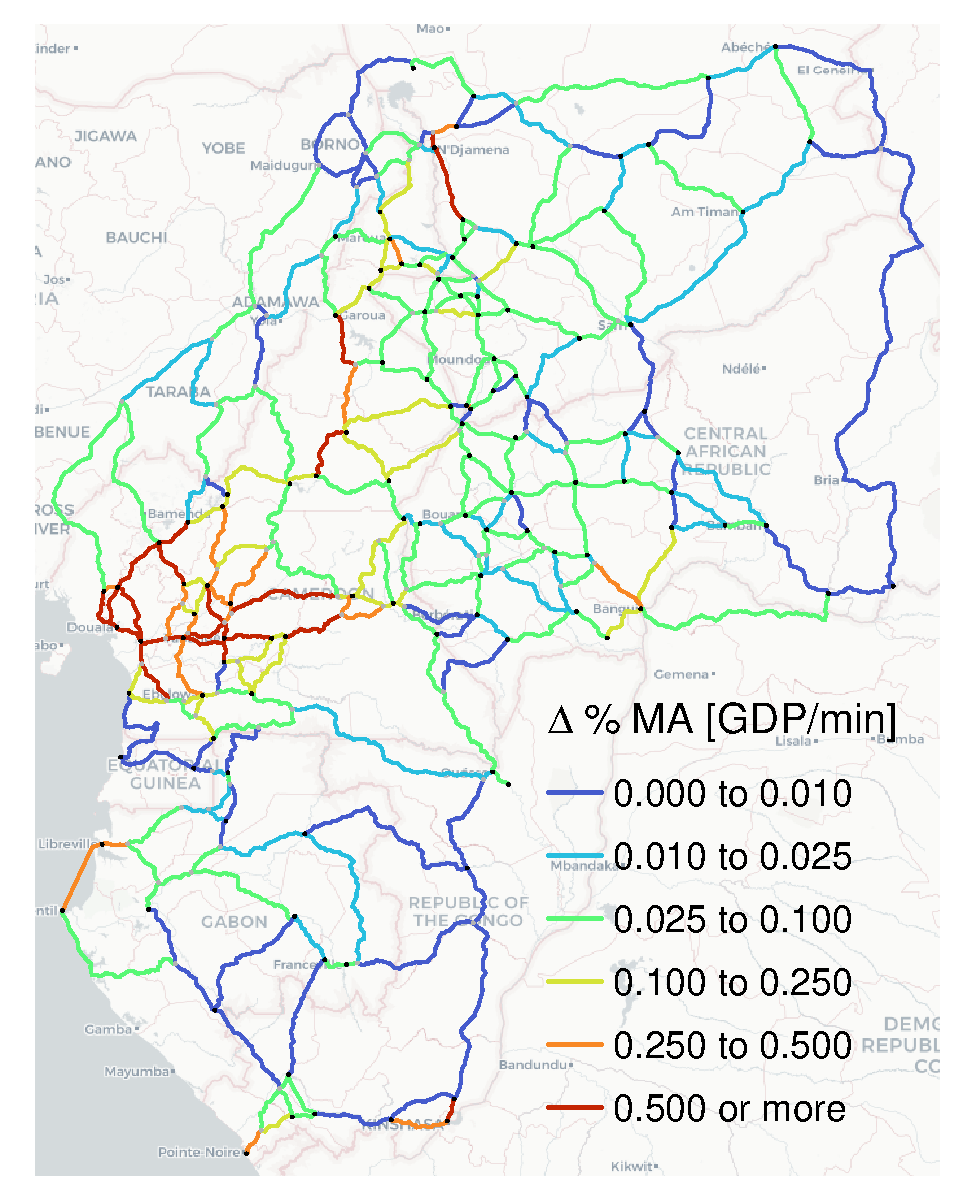
\includegraphics[width=0.38\textwidth, trim= {0.9cm 0 0.9cm 0}, clip]{"../figures/PE/trans_CEMAC_network_MACR_90_min_speed_bt_perc_google.pdf"} & 
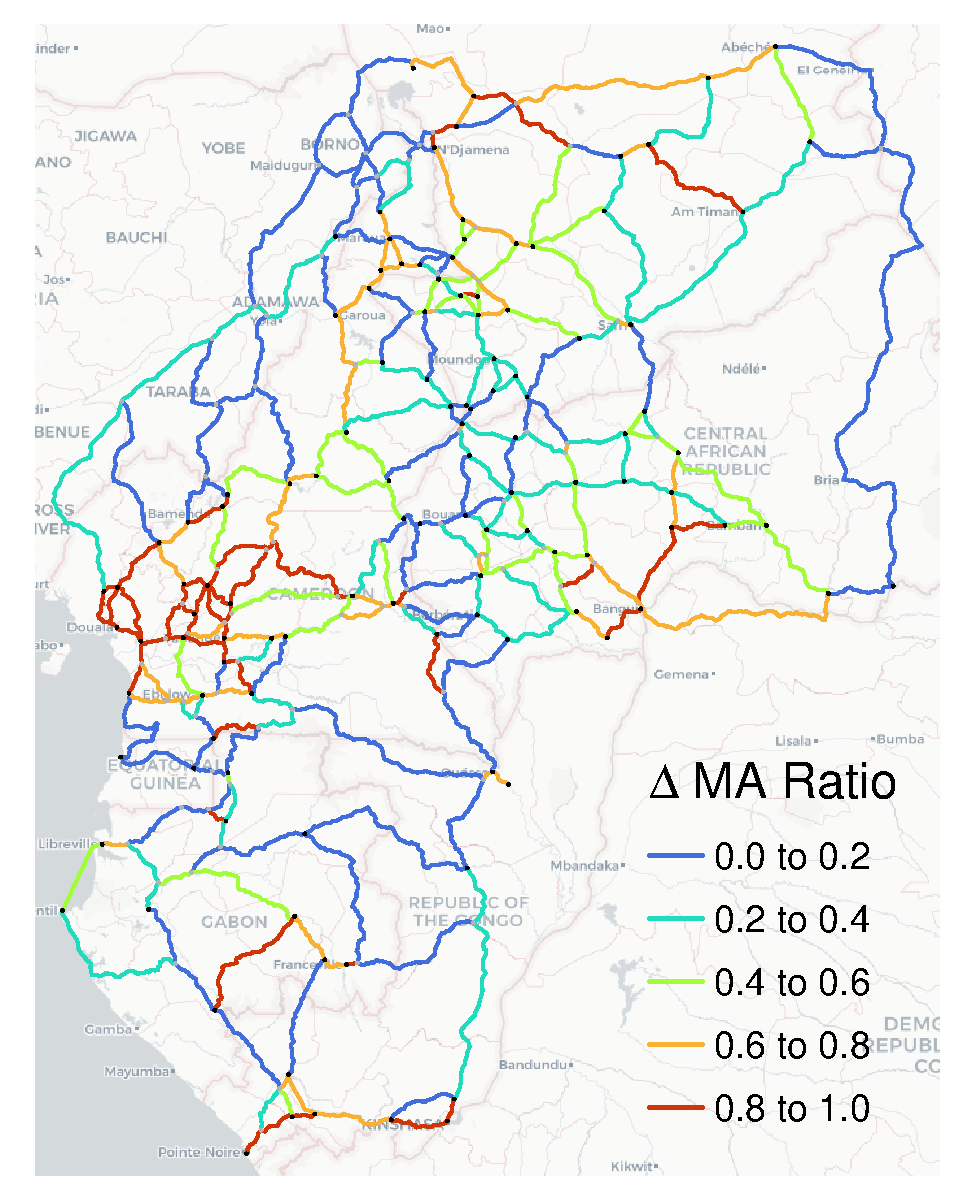
\includegraphics[width=0.38\textwidth, trim= {0.9cm 0 0.9cm 0}, clip]{"../figures/PE/trans_CEMAC_network_MACR_90_min_speed_bt_ratio_google.pdf"}
\end{tabular}
\end{adjustbox}
\end{frame}

\begin{frame}{Extending \& Upgrading Network to 90km/h - MA Returns (\$/min/\$)}
\vspace{-2mm}
All works cost \$27B (\$19B upgrading, \$8B new links) and yield \textbf{71.9.8\%} MA gain (LHS, 0.68\$/min/\$), and \textbf{67.6\%} (0.35\$/min/\$) under frictions. Median ratio: 0.42.
\begin{adjustbox}{center}
\begin{tabular}{@{}c@{}c@{}@{}c@{}} 
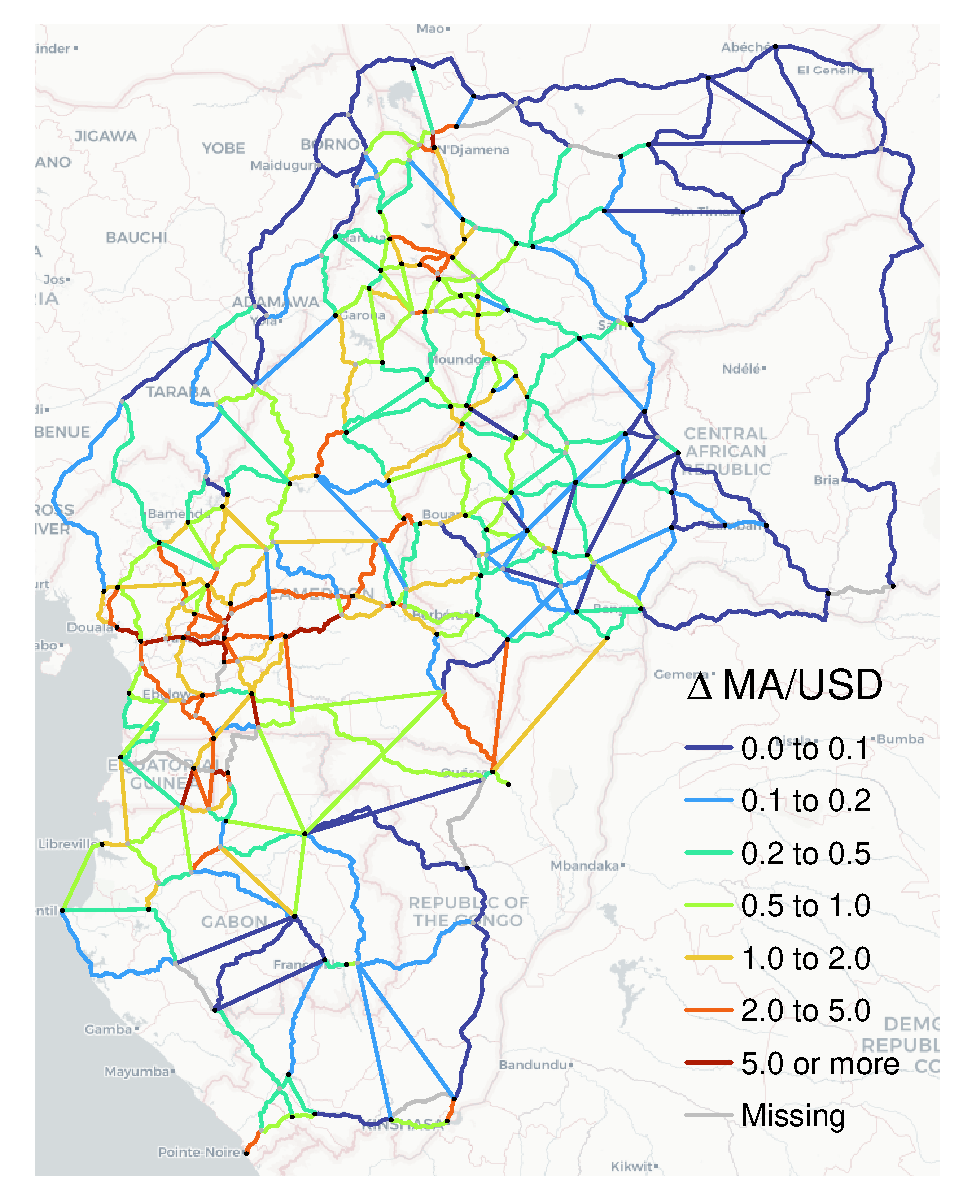
\includegraphics[width=0.38\textwidth, trim= {0.9cm 0 0.9cm 0}, clip]{"../figures/PE/trans_CEMAC_network_MACR_gain_all_90kmh_pusd_google.pdf"} & 
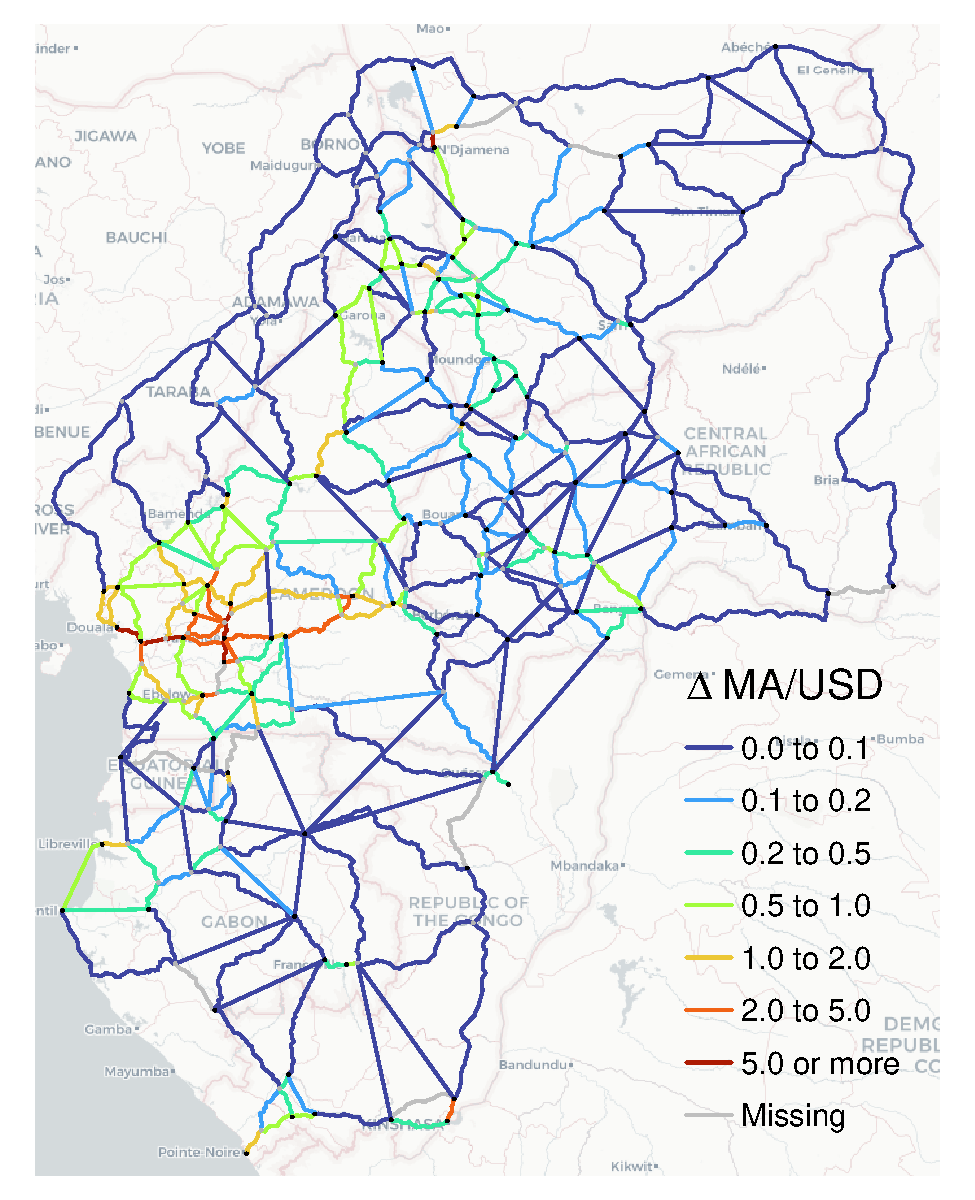
\includegraphics[width=0.38\textwidth, trim= {0.9cm 0 0.9cm 0}, clip]{"../figures/PE/trans_CEMAC_network_MACR_gain_all_90kmh_pusd_bt_google.pdf"} & 
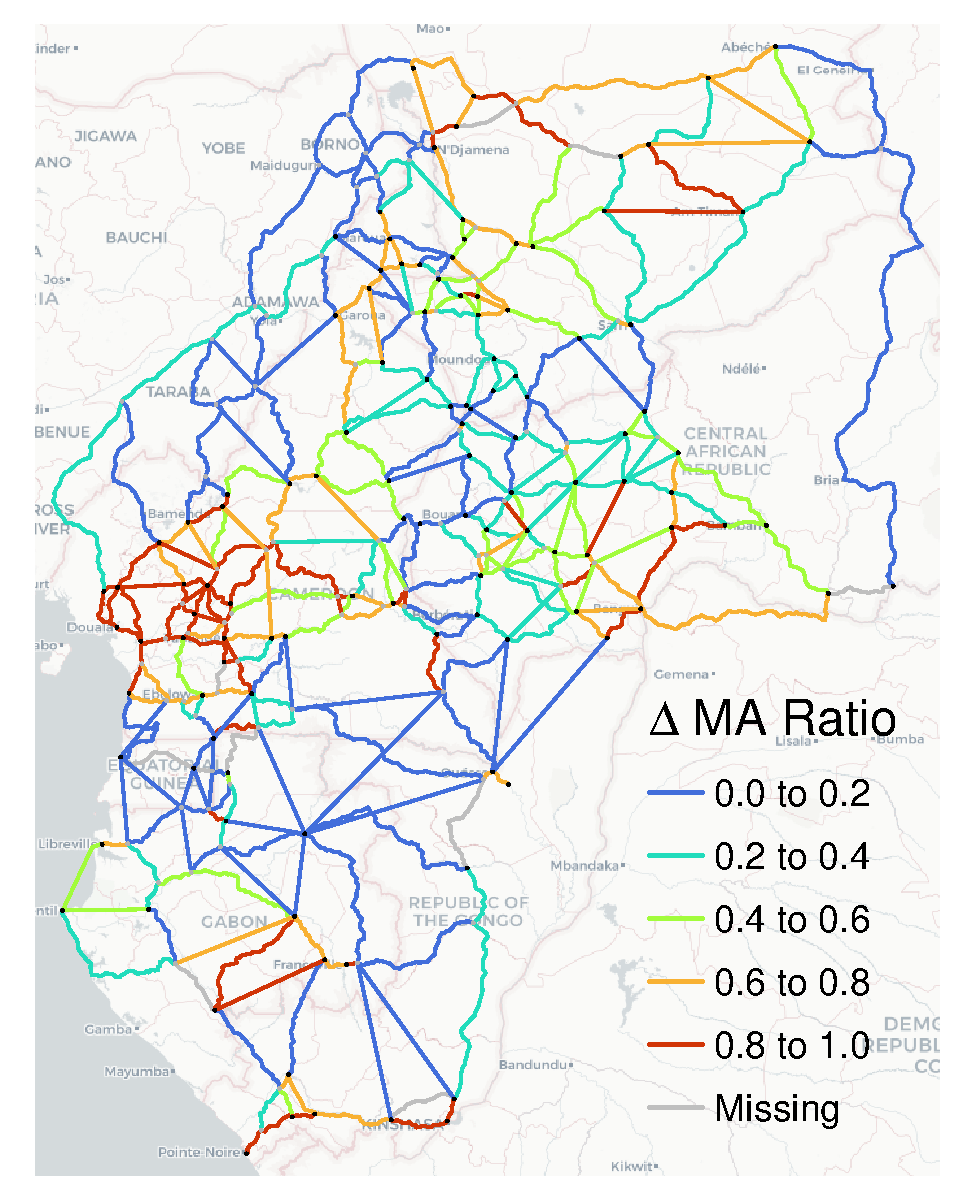
\includegraphics[width=0.38\textwidth, trim= {0.9cm 0 0.9cm 0}, clip]{"../figures/PE/trans_CEMAC_network_MACR_gain_all_90kmh_pusd_bt_ratio_google.pdf"}
\end{tabular}
\end{adjustbox}
\end{frame}

\begin{frame}{Consensus Packages (Program Selection)}
\vspace{-2.5mm}
\begin{adjustbox}{center}
\begin{tabular}{@{}c@{}|@{}c@{}|@{}c@{}} 
Average (FR/NoFR) & No Frictions & NoFR \& NoNewLinks \\
$>\$0.5$ $|$ C: 4.3 $|$ G: 2.6 (43\%) & $>\$1$ $|$ C: 5.4 $|$ G: 2.3 (49\%) & $>\$1$ $|$ C: 4 $|$ G: 2.8 (44\%) \\
Frictions G: 1.9\$/min/\$ (53\%) & Frictions G: 1.4\$/min/\$ (51\%) & Frictions G: 1.7\$/min/\$ (47\%) \\ [-0.5em]
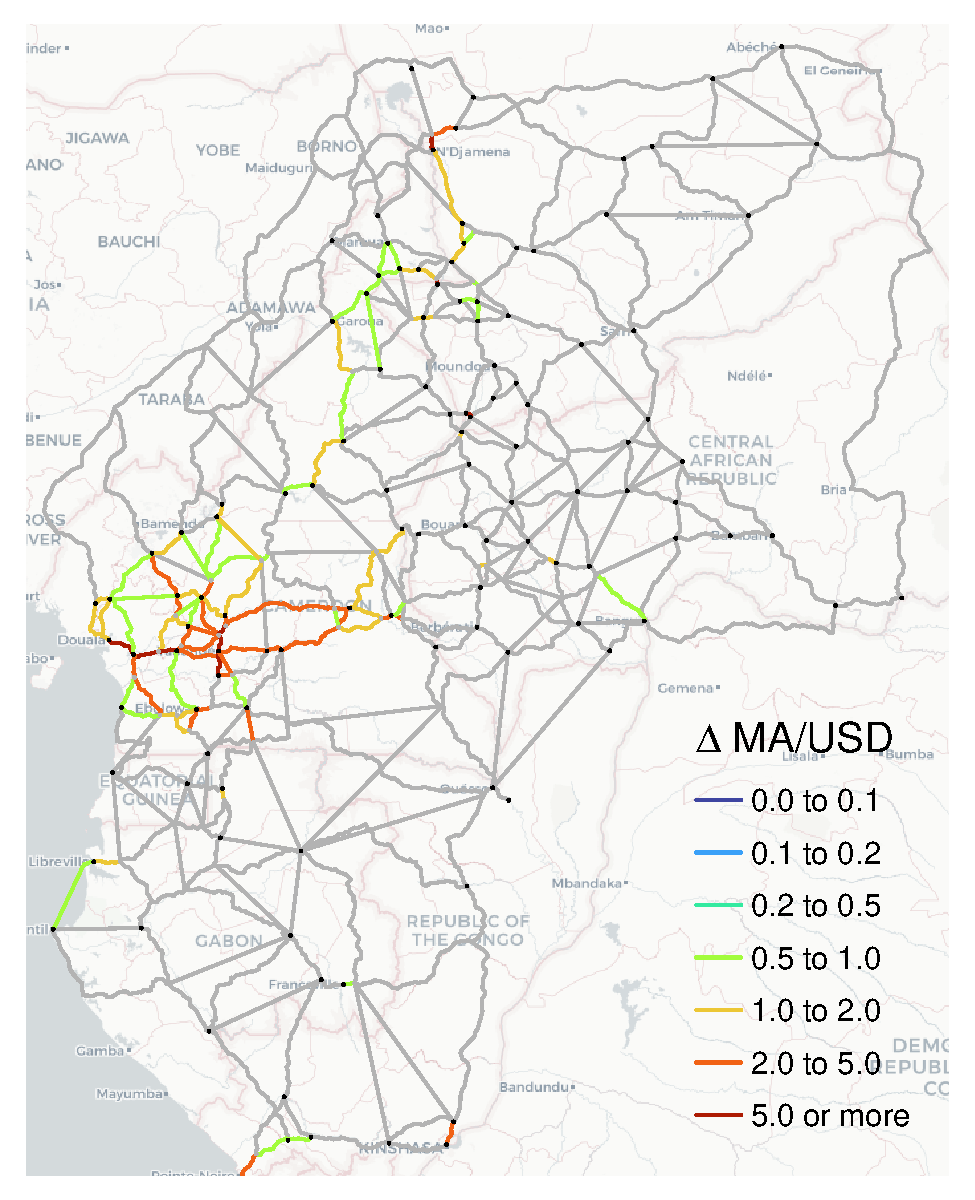
\includegraphics[width=0.38\textwidth, trim= {0.9cm 0 0.9cm 0}, clip]{"../figures/PE/trans_CEMAC_network_MACR_gain_all_90kmh_pusd_cons_MAg0.5_google.pdf"} & 
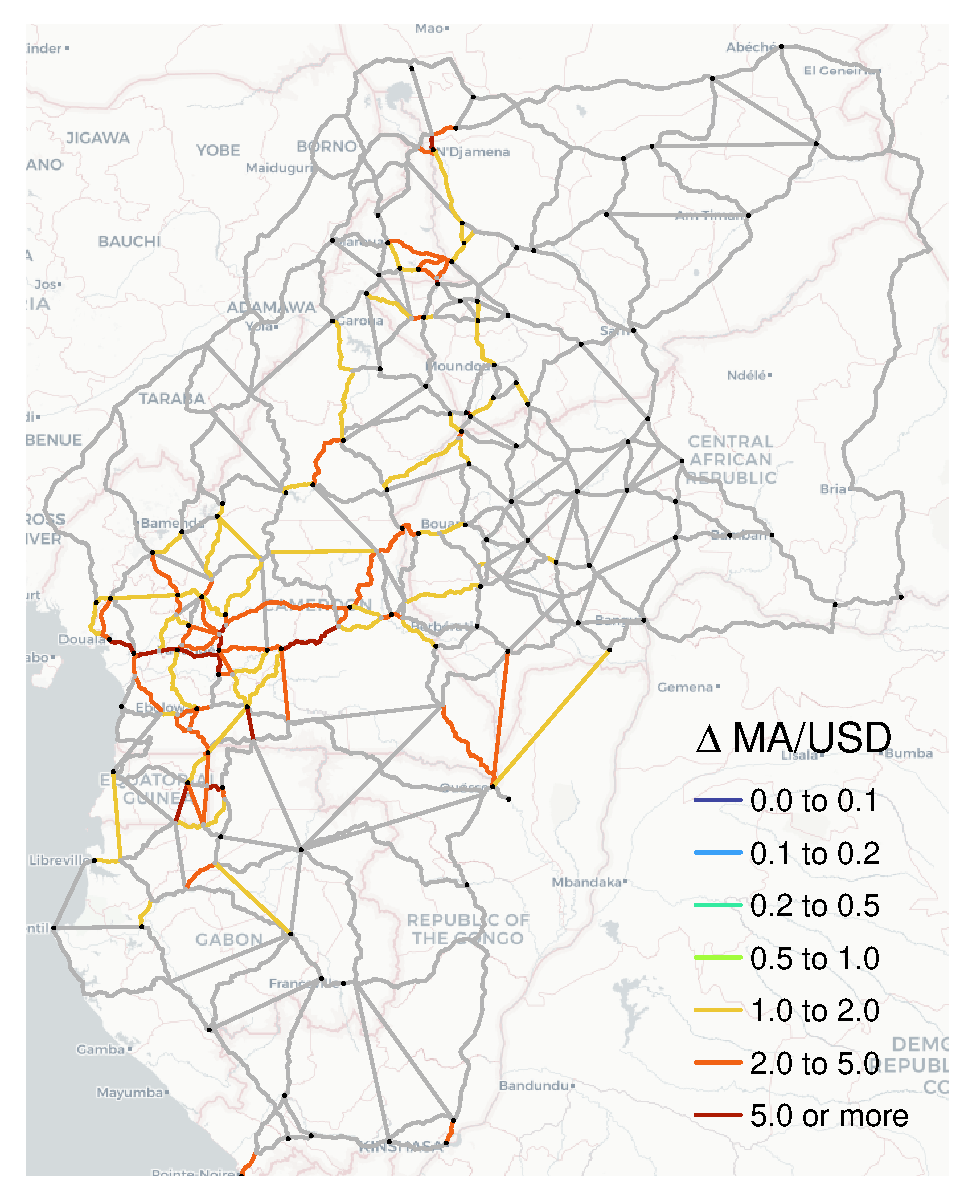
\includegraphics[width=0.38\textwidth, trim= {0.9cm 0 0.9cm 0}, clip]{"../figures/PE/trans_CEMAC_network_MACR_gain_all_90kmh_pusd_cons_nofr_MAg1_google.pdf"} &
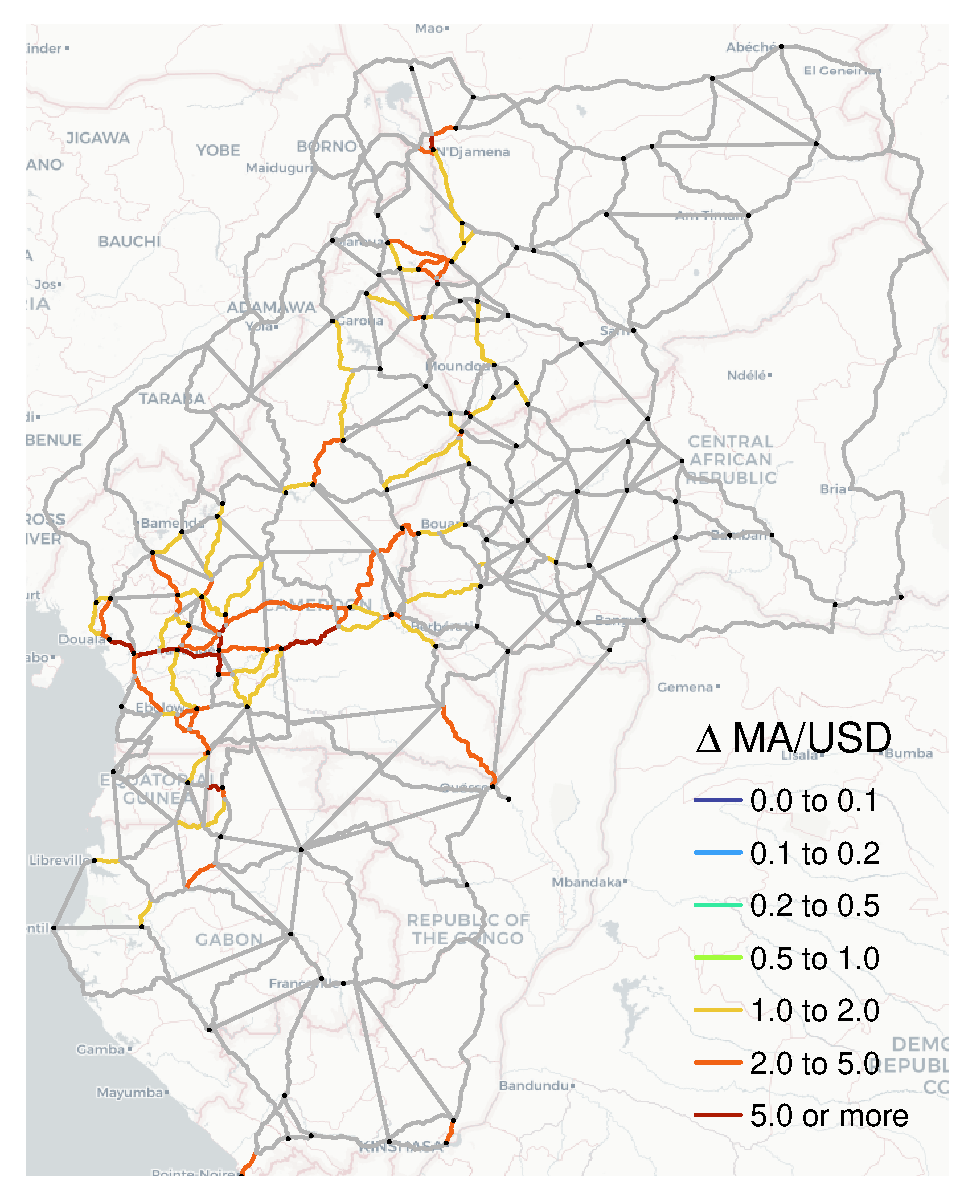
\includegraphics[width=0.38\textwidth, trim= {0.9cm 0 0.9cm 0}, clip]{"../figures/PE/trans_CEMAC_network_MACR_gain_all_90kmh_pusd_cons_nofr_noadd_MAg1_google.pdf"}  
\end{tabular}
\end{adjustbox}
\end{frame}

\begin{frame}{Border Post Optimization}
\vspace{-2mm}
Three Scenarios: Border time reduction by 50\% following \citet{fontagne2023trade} (LHS) or to 12h (middle, 90\% reduction from median), or by 100\% (RHS, set to zero). 
\begin{adjustbox}{center}
\begin{tabular}{@{}c@{}c@{}@{}c@{}} 
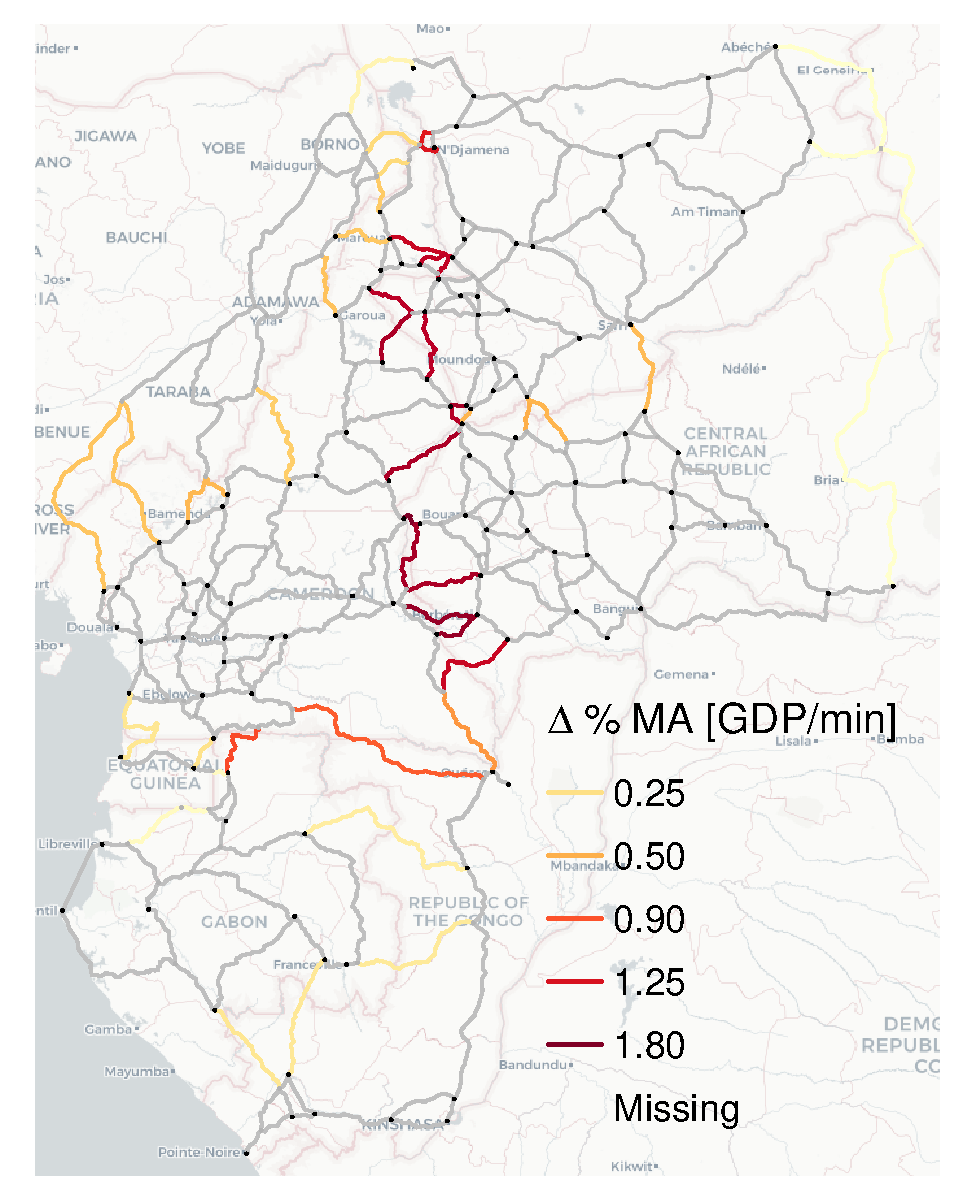
\includegraphics[width=0.38\textwidth, trim= {0.9cm 0 0.9cm 0}, clip]{"../figures/PE/trans_CEMAC_network_MACR_bt_50perc_red_perc_google.pdf"} & 
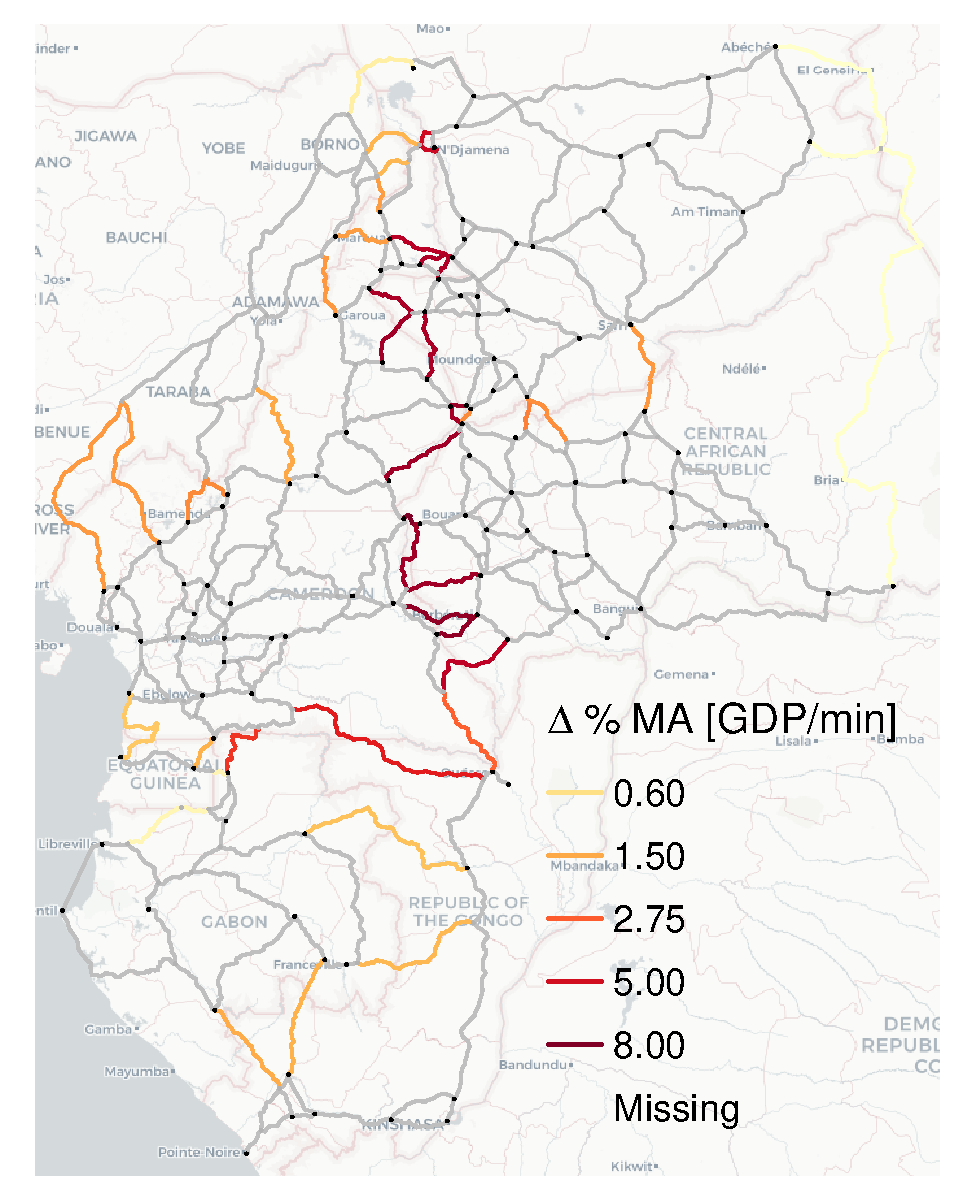
\includegraphics[width=0.38\textwidth, trim= {0.9cm 0 0.9cm 0}, clip]{"../figures/PE/trans_CEMAC_network_MACR_bt_90percto12h_red_perc_google.pdf"} & 
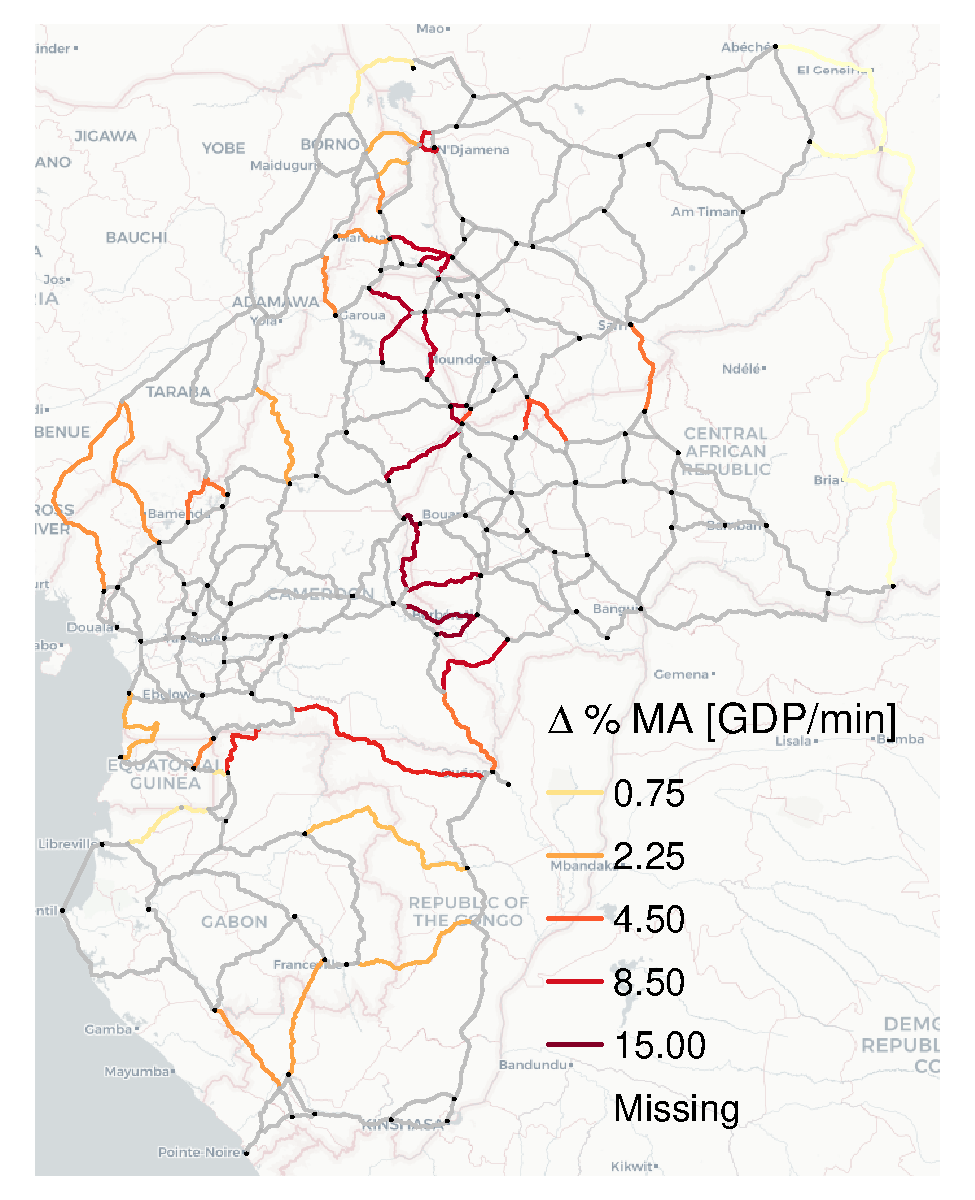
\includegraphics[width=0.38\textwidth, trim= {0.9cm 0 0.9cm 0}, clip]{"../figures/PE/trans_CEMAC_network_MACR_bt_100perc_red_perc_google.pdf"}
\end{tabular}
\end{adjustbox}
\end{frame}

\begin{frame}{Macroeconomic Cost-Benefit Analysis}
How do MA gains translate into economic gains? \citet{donaldson2016railroads} regress ln(US land values) on ln(MA) and find elasticity $\sim$\textbf{0.5}. But Africa $\neq$ US.\\ \vspace{3mm}

\textbf{Question}: What assumption about \%$\Delta$MA $\to$ \%$\Delta$\%$\Delta$GDP needed to break even? \\ \vspace{2mm}
\begin{itemize} \setlength{\itemsep}{0.7em}
\item CEMAC GDP in 2023 was \textbf{90.9} billion 2015 USD. Median growth rate in 2000-2023 was \textbf{3.5\%}. If we are pessimistic: \textbf{2\%} going forward. 
\item Discount the future by \textbf{10\%} [MSCI World $\sim$8\%, JP Morgan EMBI $\sim$6\%] 
\item Cutoff after \textbf{30} years.
\end{itemize} \vspace{3mm}
% Then, we can evaluate the scenarios as follows:
\begin{adjustbox}{center}
\begin{tabular}{lrrrr}
\textbf{Work Package} & \textbf{Cost} & \textbf{\%$\Delta$MA} & \textbf{BEG} (3.5\%) & \textbf{BEG} (2\%) \\ \midrule
All Works & \$27B  & $68-72$ &  5.79\% $\to$ 3.703 & 12.7\% $\to$ 2.253 \\
All Upgrades & \$19B  & $60-64$ &  4.10\% $\to$ 3.643 & 8.96\% $\to$ 2.179 \\
Links $>\$0.5$/min/\$ (Avg) & \$4.3B & $43-53$ & 0.94\% $\to$ 3.533 & 2.05\% $\to$ 2.041 \\
Links $>\$1$/min/\$ (NoFR) & \$5.4B & $49-51$ & 1.17\% $\to$ 3.541 & 2.57\% $\to$ 2.051 \\
All Links $>\$1$/min/\$ (NFNN) & \$4B & $44-47$ & 0.87\% $\to$ 3.530 & 1.91\% $\to$ 2.038
\end{tabular}
\end{adjustbox}
\end{frame}


%------------------------------------------------
\section{Optimal Investments in General Equilibrium}
%------------------------------------------------

\sectionframe{Optimal Investments in General Equilibrium}

\begin{frame}[label=GEModel]{Optimal Transport Networks in Spatial Equilibrium \quad \hyperlink{GEModelSol}{\beamergotobutton{model solution}}}
\setlength{\abovedisplayskip}{2pt}
\setlength{\belowdisplayskip}{2pt}
\vspace{-2mm}
\citet{fajgelbaum2020optimal} nest optimal allocation and network flow problems into a global network design problem and compute welfare maximizing transport networks:
\begin{equation}
\max_{c_j,h_j,C_j^n,L_j^n,Q_{jk}^n,I_{jk}} \sum_{j} \omega_j L_j U (c_j, h_j)
\end{equation}
with $U (c,h) = c^\alpha h^{1-\alpha}$, s.t. availability of (non-)traded goods and balanced flows
\begin{equation}
c_j L_j \leq \left[ \sum_{n=1}^{N} (C_j^n)^{\frac{\sigma-1}{\sigma}} \right]^{\frac{\sigma}{\sigma-1}}, \sigma > 1,\quad\forall\ j; \qquad h_j L_j \leq H_j\quad\forall\ j;
\end{equation}
\begin{equation} \label{eq:BALFL}
C_j^n + \sum_{k \in N(j)} \left(1 + \tau_{jk} (Q_{jk}^n, I_{jk}) \right) Q_{jk}^n \leq Z_j^n (L_j^n)^\alpha + \sum_{k \in N(j)} Q_{kj}^n\quad\forall\ j,n
\end{equation}
with per unit shipping cost $\tau_{jk} (Q_{jk}^n, I_{jk}) = \delta^\tau_{jk} (Q_{jk}^n)^\beta I_{jk}^{-\gamma}$, a network-building constraint, exogenous network bounds, infrastructure symmetry, local labor market clearing
\begin{equation} 
\sum_{j} \sum_{k \in N(j)} \delta^I_{jk} I_{jk} \leq K; \quad 0 \leq \underline{I}_{jk} \leq I_{jk} \leq \overline{I}_{jk};\quad I_{jk} = I_{kj};\quad \sum_{n=1}^N L^n_j\leq L_j\quad\forall\ j;
\end{equation}
and the non-negativity of $c_j$, $C^n_j$, $L^n_j$, $I_{jk}$, and $Q^n_{jk}$.
\end{frame}


\begin{frame}{Parameterization for GE Simulations} 
\begin{adjustbox}{center}
    \begin{columns} \setlength{\columnsep}{0.5mm} % Set the space between columns to 1 cm
        % Left column
                \begin{column}{0.015\textwidth}
                \end{column}
        \begin{column}{0.33\textwidth} \scriptsize 
\setlength{\abovedisplayskip}{6pt} % Space above equations
\setlength{\belowdisplayskip}{6pt} % Space below equations
\setlength{\parindent}{0pt} % Disable paragraph indentation
\hphantom{.}\\ \vspace{-3mm}
20 different products (largest 16 cities own). $\sigma = 3.8$ \citep{bajzik2020estimating}, $Z_j^\text{city} = \text{GDP}_j/\text{Population}_j$, 
$$Z_j^{\text{port}} = \frac{2100 \times \text{Outflow}_j}{\text{Population}_j}.\ (\text{16\%})$$
Following \citet{graff2024spatial}: $\alpha=0.7$, $\beta = 1.177$, and $\gamma = 0.946$ (DRS).
$$ \text{I}_{jk} = \text{speed (km/h)}_{jk} \ \ \forall\, j,k,$$
$\underline{I}_{jk} = \text{I}_{jk}$, $\overline{I}_{jk} = \max(I_{jk}, 90)$. Per km/h infrastructure building cost $\delta^\text{I}_{jk}$:
$$\delta^\text{I}_{jk} = \text{upgrade cost}_{jk} / (\overline{I}_{jk} - \text{I}_{jk}) \ \ \forall\, j,k.$$
Baseline budget is $K_0 = \delta^\text{I}_{jk}\times I_{jk}$. Planner given $K_0+\$1\text{B}/\$2\text{B}/\$4\text{B}$. 
Iceberg trade costs \citep{graff2024spatial}: 
 $$\delta^\tau_{jk} = 0.1159 \times \ln(\text{distance in miles}_{jk}).$$
        \end{column}
        % Right column
        \begin{column}{0.8\textwidth}
\resizebox{\textwidth}{!}{
\begin{tabular}{@{}c@{}c@{}}
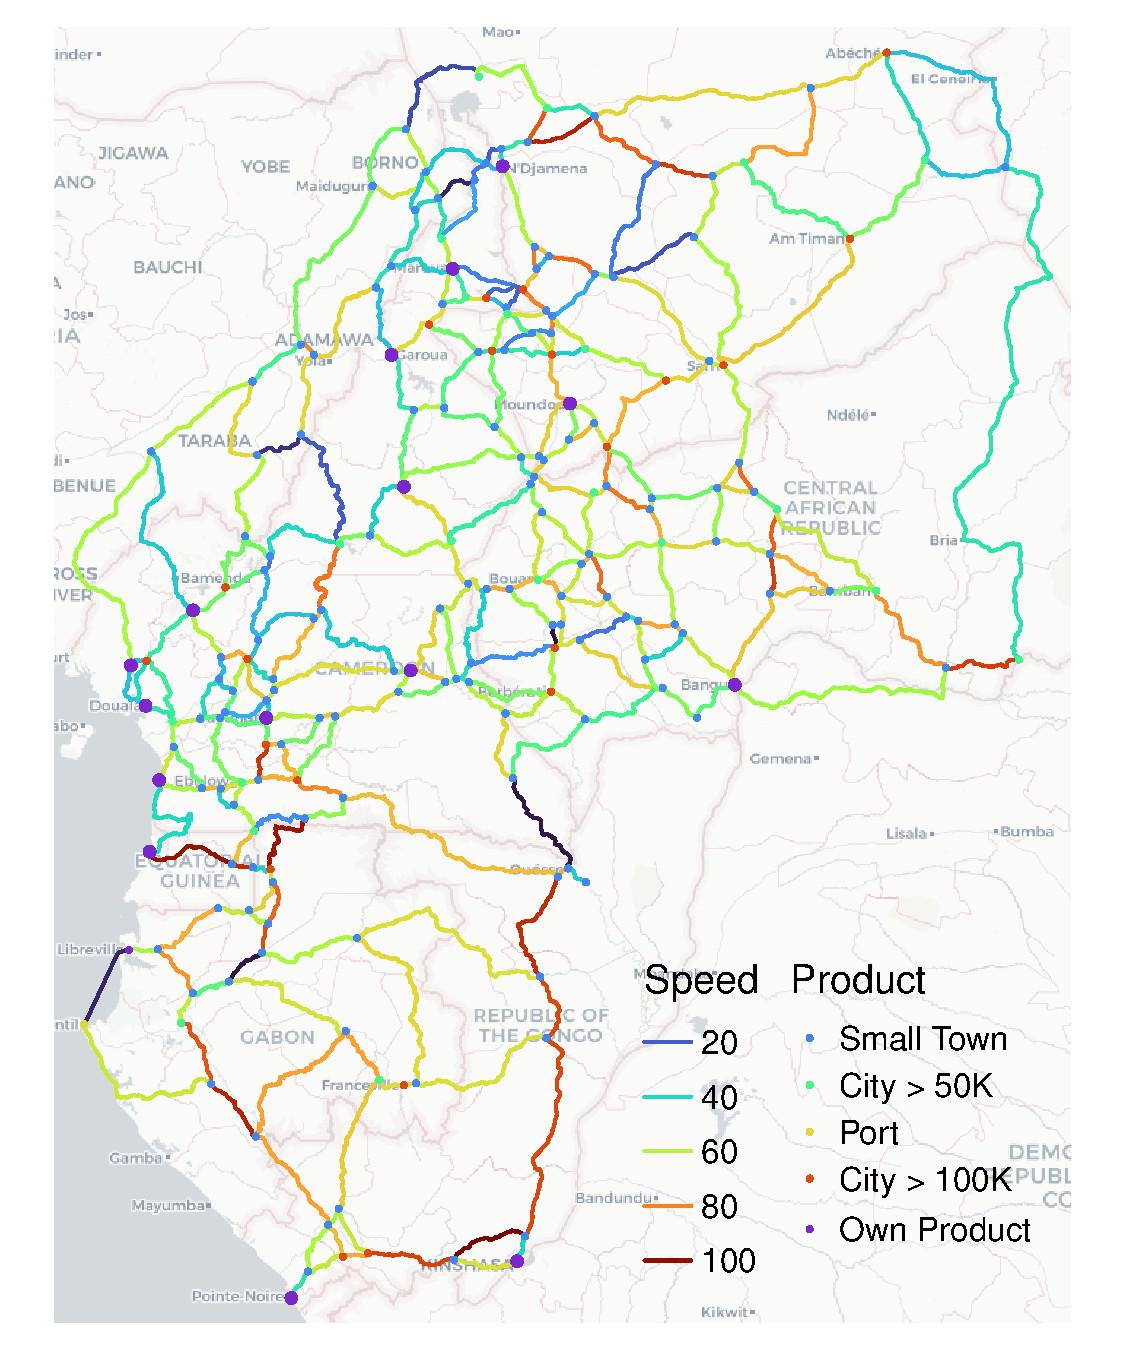
\includegraphics[width=0.5\textwidth, trim= {11.8mm 0mm 11mm 0mm}, clip]{"../figures/GE/trans_africa_network_reduced_20_products_google.pdf"} & 
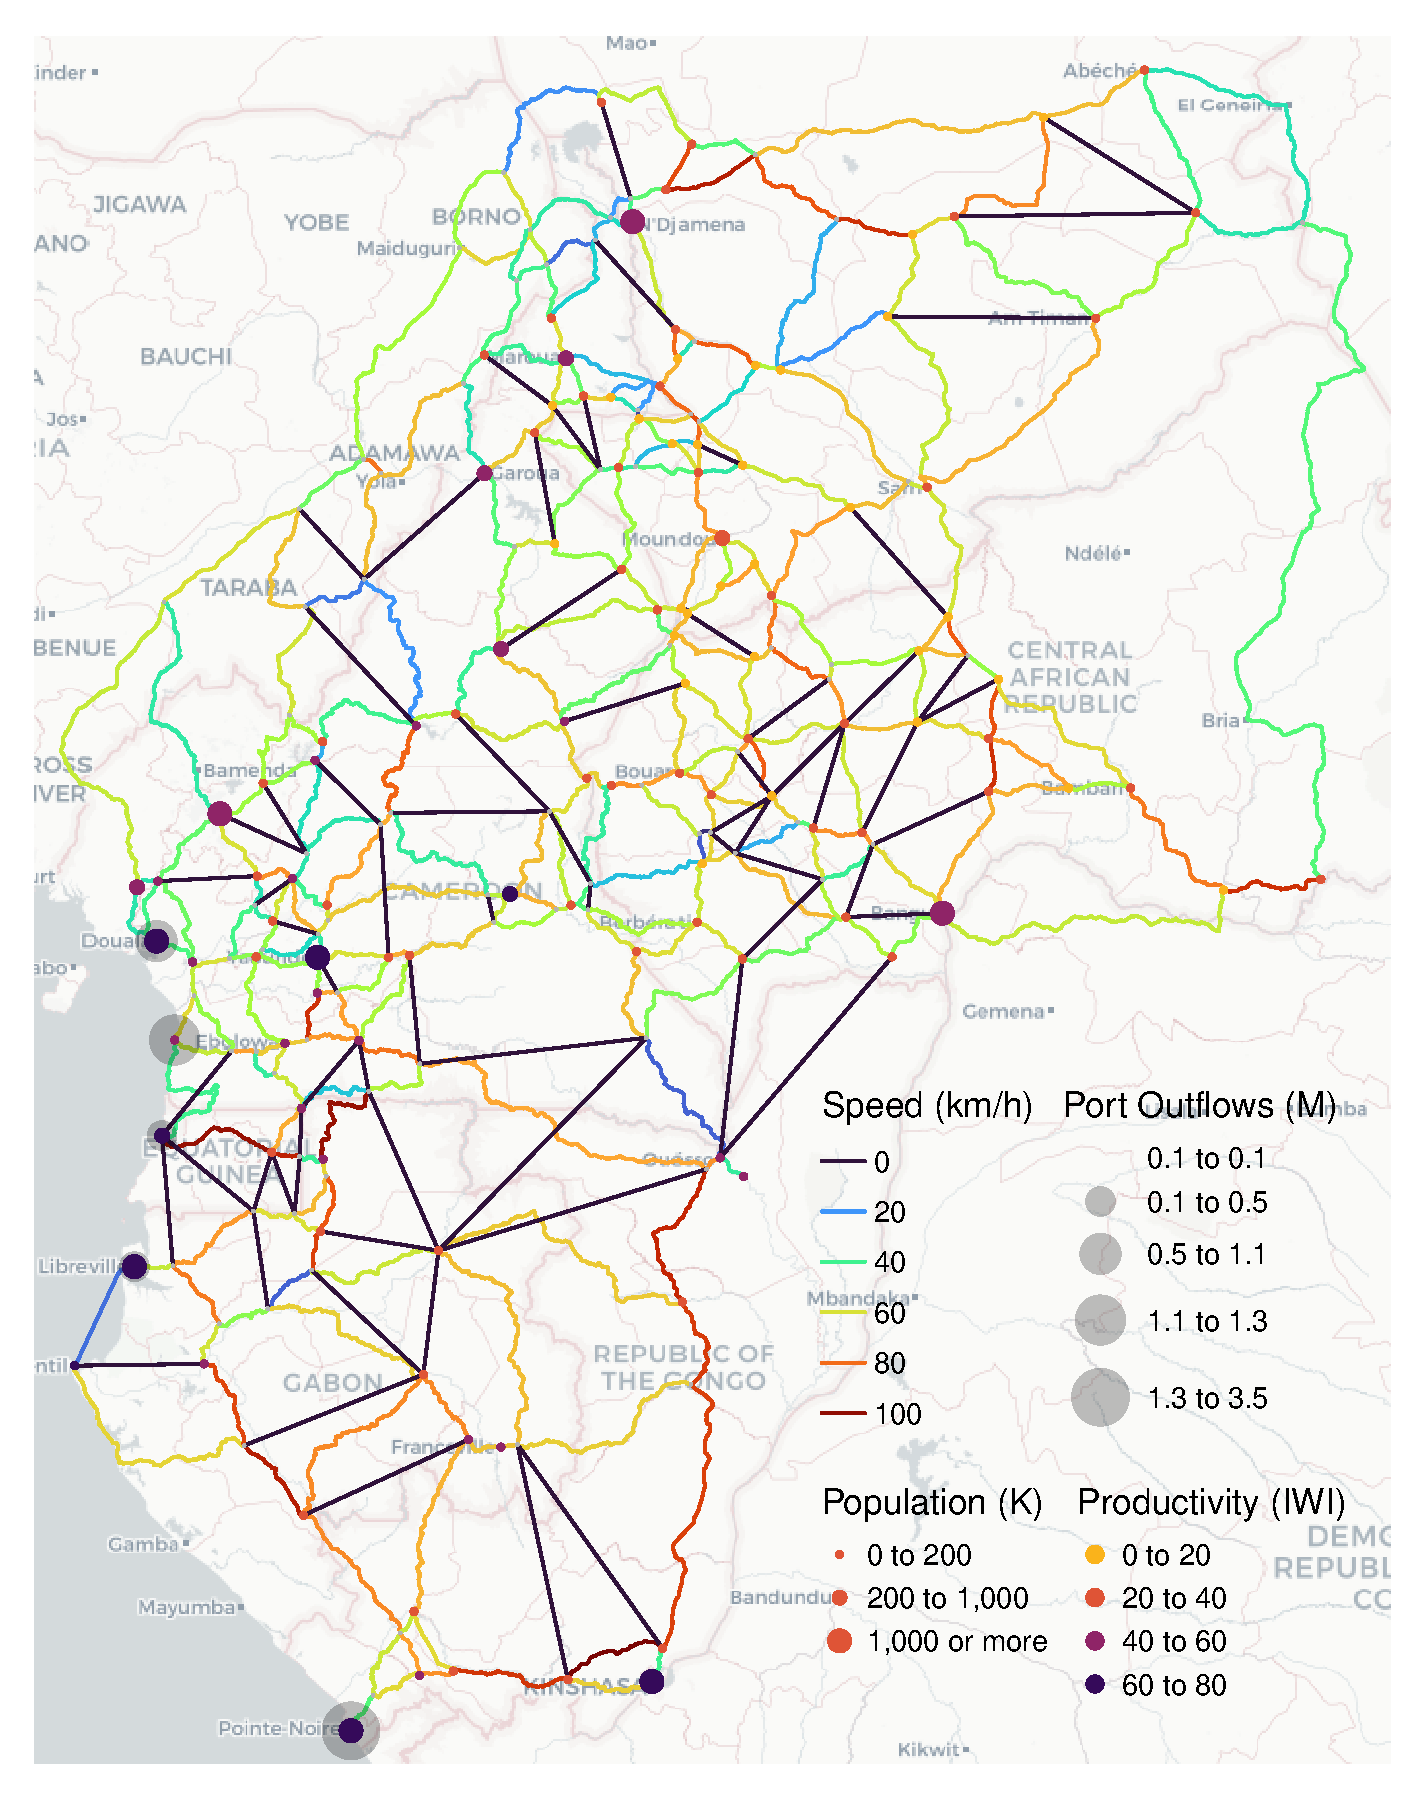
\includegraphics[width=0.5\textwidth, trim= {9mm 0 9mm 0}, clip]{"../figures/trans_CEMAC_network_GE_parameterization_latest_google.pdf"}
\end{tabular}
}
        \end{column}
    \end{columns}
  \end{adjustbox}
\end{frame}


\begin{frame}[label=IOU]{Optimal Allocations - Only Upgrades \quad \hyperlink{EXPOU}{\beamergotobutton{exports}}}
\vspace{-1mm}
\begin{adjustbox}{center}
\begin{tabular}{@{}c@{}|@{}c@{}|@{}c@{}} 
\$1B USD'15 & \$2B USD'15 & \$4B USD'15 \\
Upgraded: 1543km & Upgraded: 3152km & Upgraded: 6905km \\ 
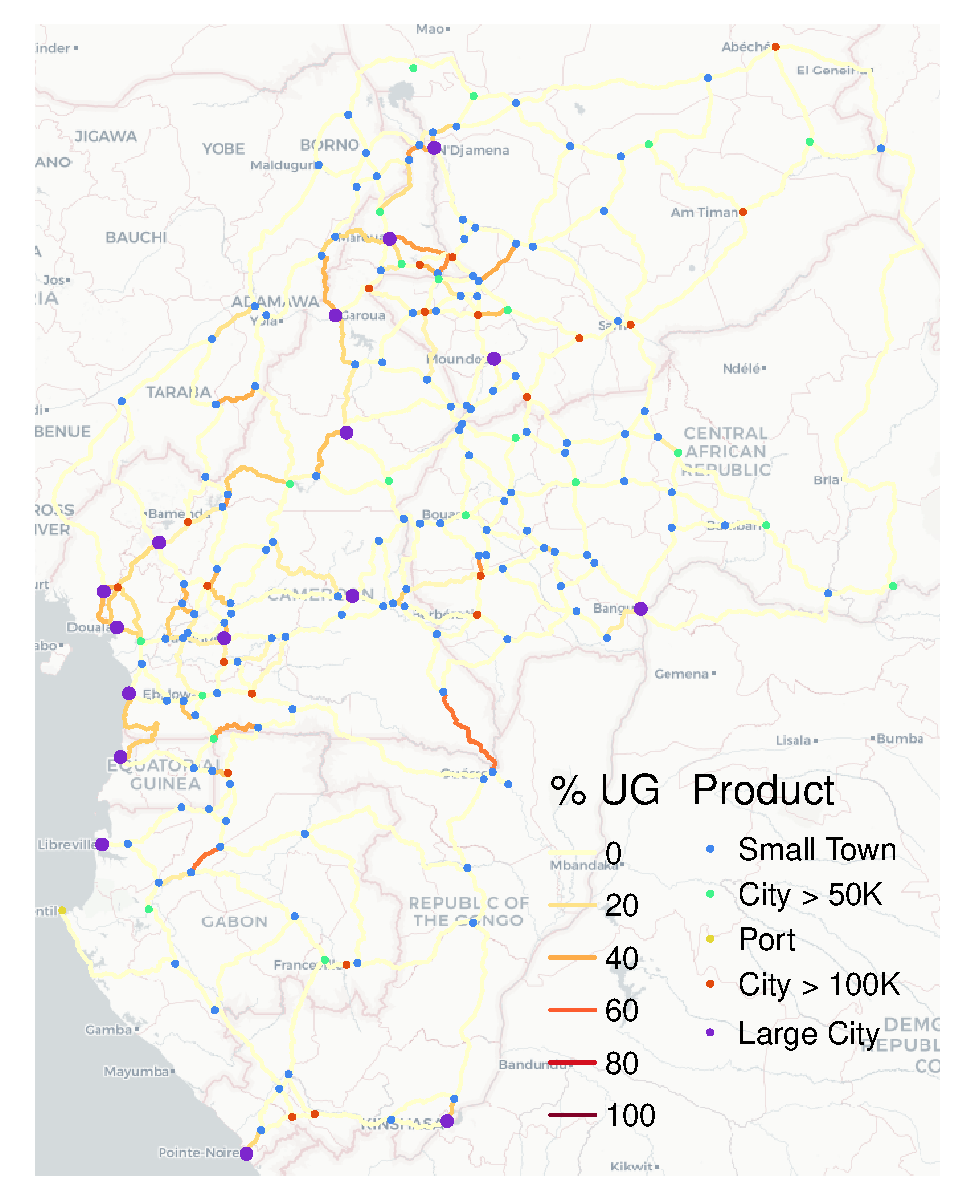
\includegraphics[width=0.38\textwidth, trim= {0.9cm 0 0.9cm 0}, clip]{"../figures/GE/trans_africa_network_GE_20g_1b_fixed_cgc_sigma3.8_rho0_julia_MACR_90kmh_google_perc_ug.pdf"} & 
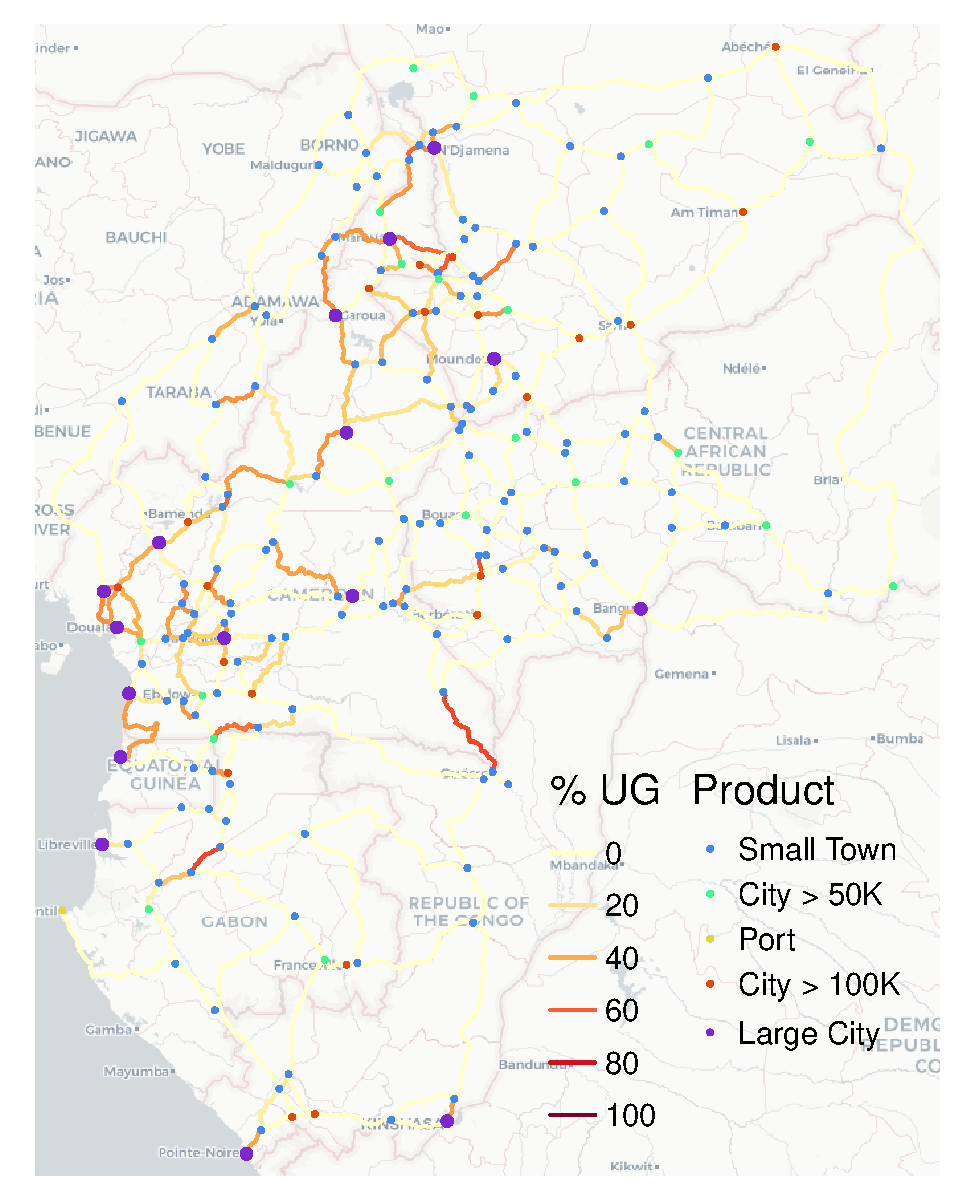
\includegraphics[width=0.38\textwidth, trim= {0.9cm 0 0.9cm 0}, clip]{"../figures/GE/trans_africa_network_GE_20g_2b_fixed_cgc_sigma3.8_rho0_julia_MACR_90kmh_google_perc_ug.pdf"} &
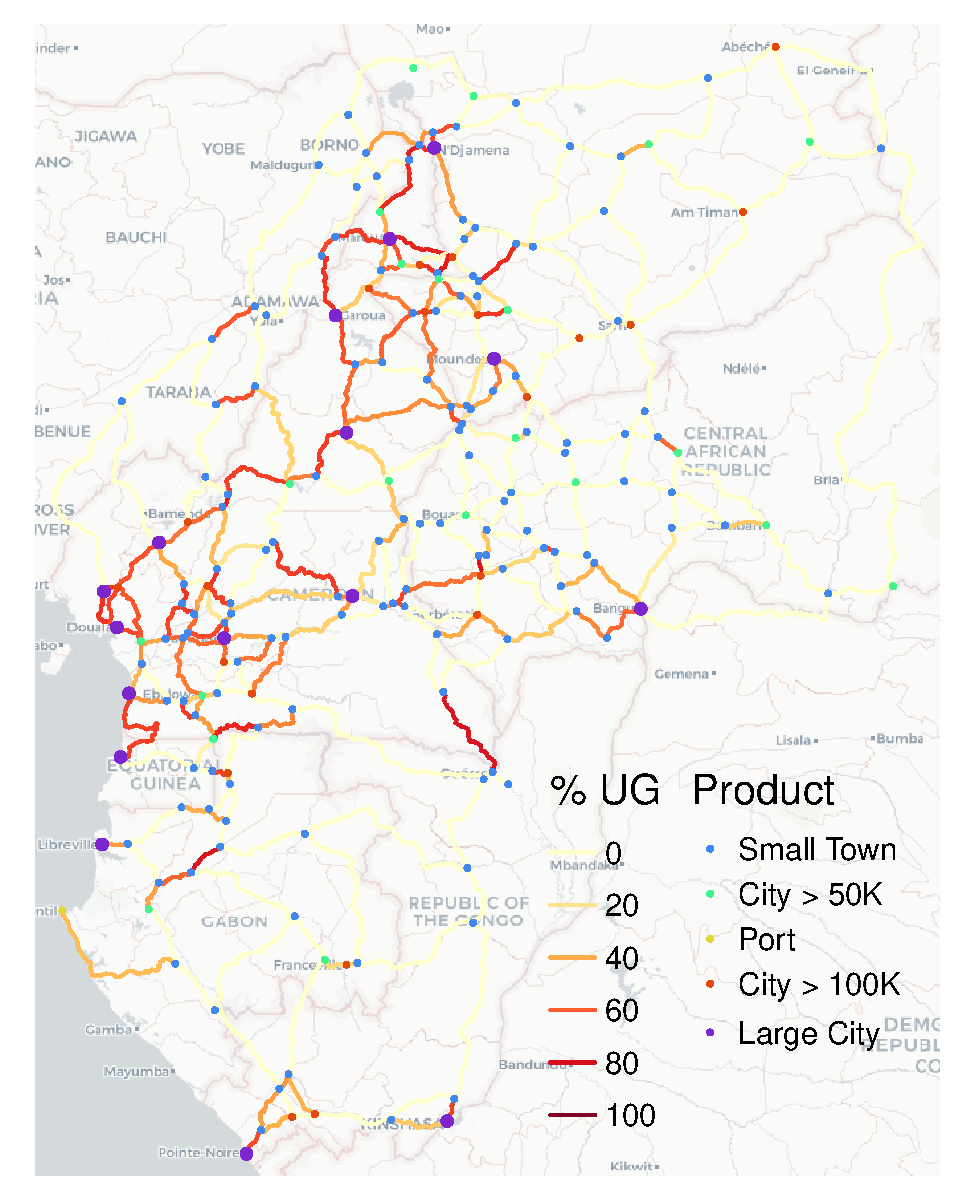
\includegraphics[width=0.38\textwidth, trim= {0.9cm 0 0.9cm 0}, clip]{"../figures/GE/trans_africa_network_GE_20g_4b_fixed_cgc_sigma3.8_rho0_julia_MACR_90kmh_google_perc_ug.pdf"}  
\end{tabular}
\end{adjustbox}
\end{frame}

\begin{frame}{Optimal Allocations - Only Upgrades - Inequality Aversion ($\rho = 2$)}
\vspace{-1mm}
\begin{adjustbox}{center}
\begin{tabular}{@{}c@{}|@{}c@{}|@{}c@{}} 
\$1B USD'15 & \$2B USD'15 & \$4B USD'15 \\
Upgraded: 1530km & Upgraded: 3085km & Upgraded: 6562km \\ 
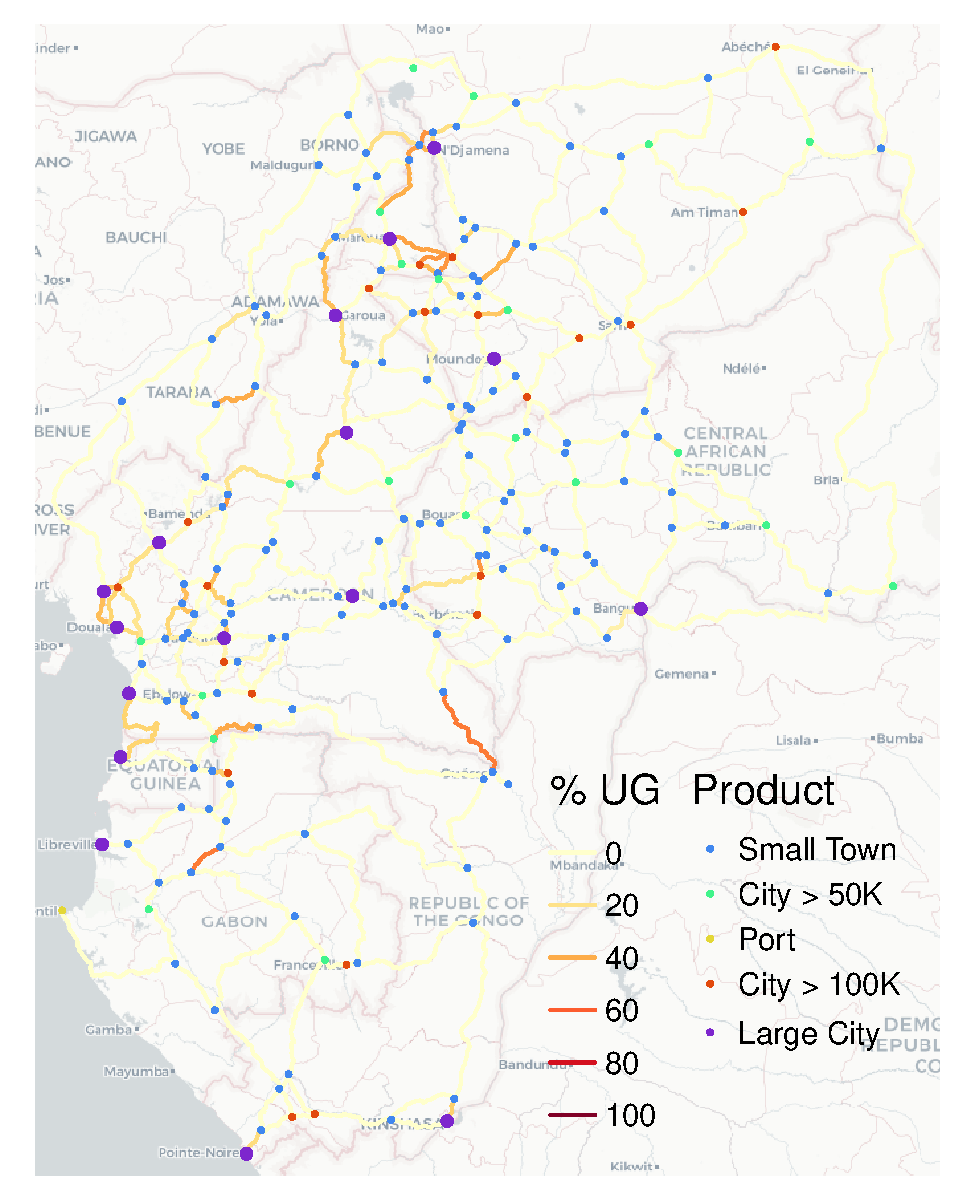
\includegraphics[width=0.38\textwidth, trim= {0.9cm 0 0.9cm 0}, clip]{"../figures/GE/trans_africa_network_GE_20g_1b_fixed_cgc_sigma3.8_rho2_julia_MACR_90kmh_google_perc_ug.pdf"} & 
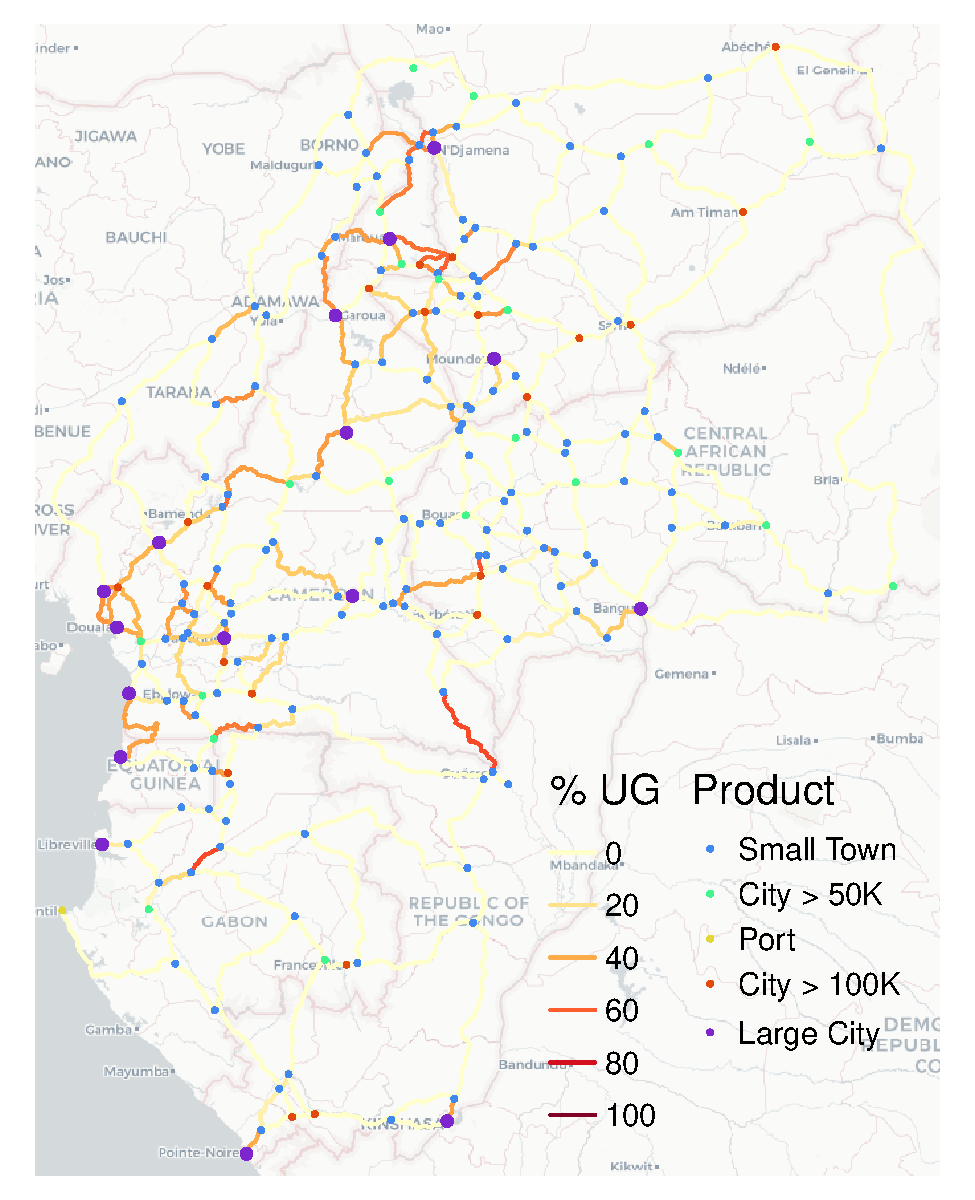
\includegraphics[width=0.38\textwidth, trim= {0.9cm 0 0.9cm 0}, clip]{"../figures/GE/trans_africa_network_GE_20g_2b_fixed_cgc_sigma3.8_rho2_julia_MACR_90kmh_google_perc_ug.pdf"} &
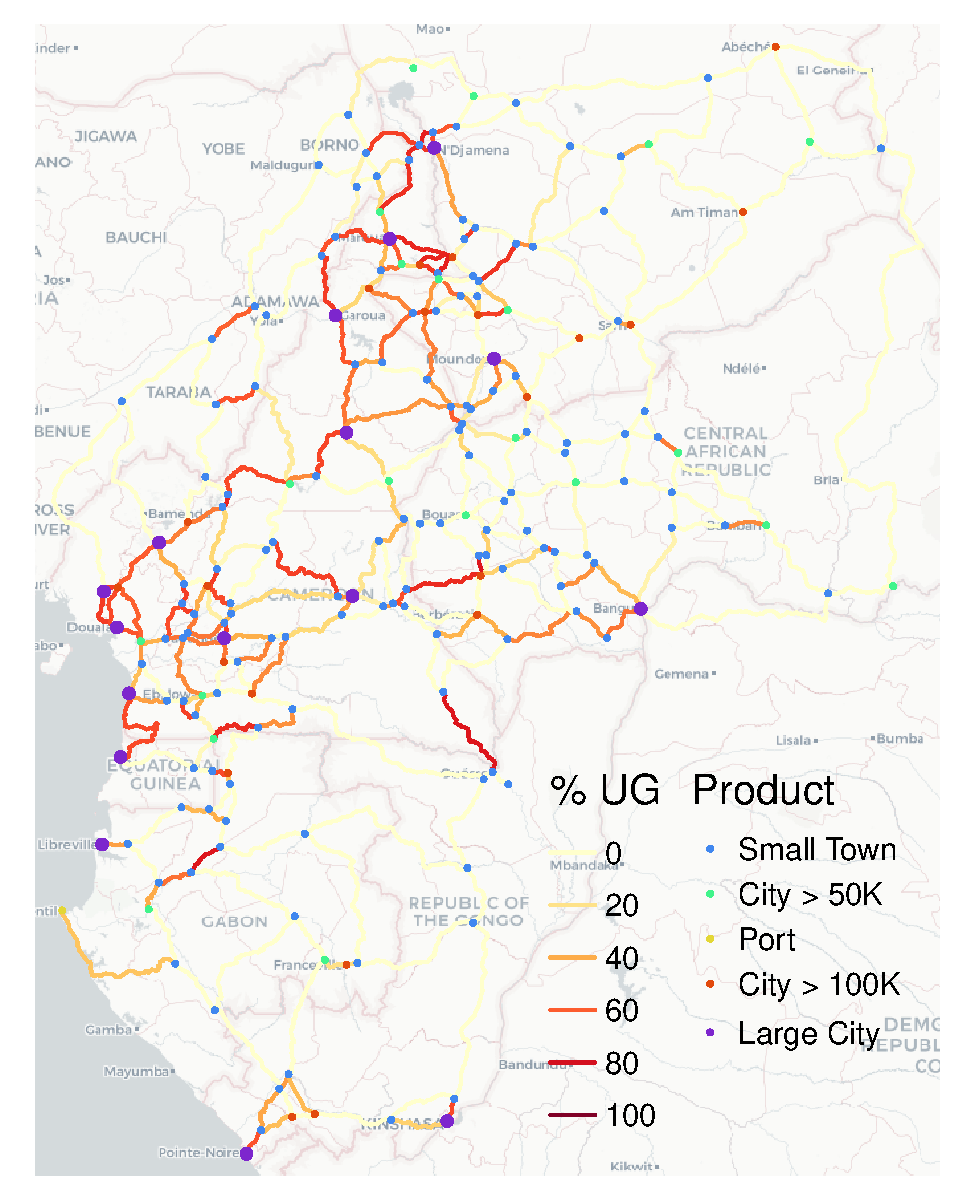
\includegraphics[width=0.38\textwidth, trim= {0.9cm 0 0.9cm 0}, clip]{"../figures/GE/trans_africa_network_GE_20g_4b_fixed_cgc_sigma3.8_rho2_julia_MACR_90kmh_google_perc_ug.pdf"}  
\end{tabular}
\end{adjustbox}
\end{frame}

\begin{frame}[label=III]{Optimal Allocations \quad \hyperlink{EXP}{\beamergotobutton{exports}}}
\vspace{-1mm}
\begin{adjustbox}{center}
\begin{tabular}{@{}c@{}|@{}c@{}|@{}c@{}} 
\$1B USD'15 & \$2B USD'15 & \$4B USD'15 \\
New: 1607km $|$ UG: 116km & New: 2943km $|$ UG: 416km & New: 4894km $|$ UG: 1713km \\ 
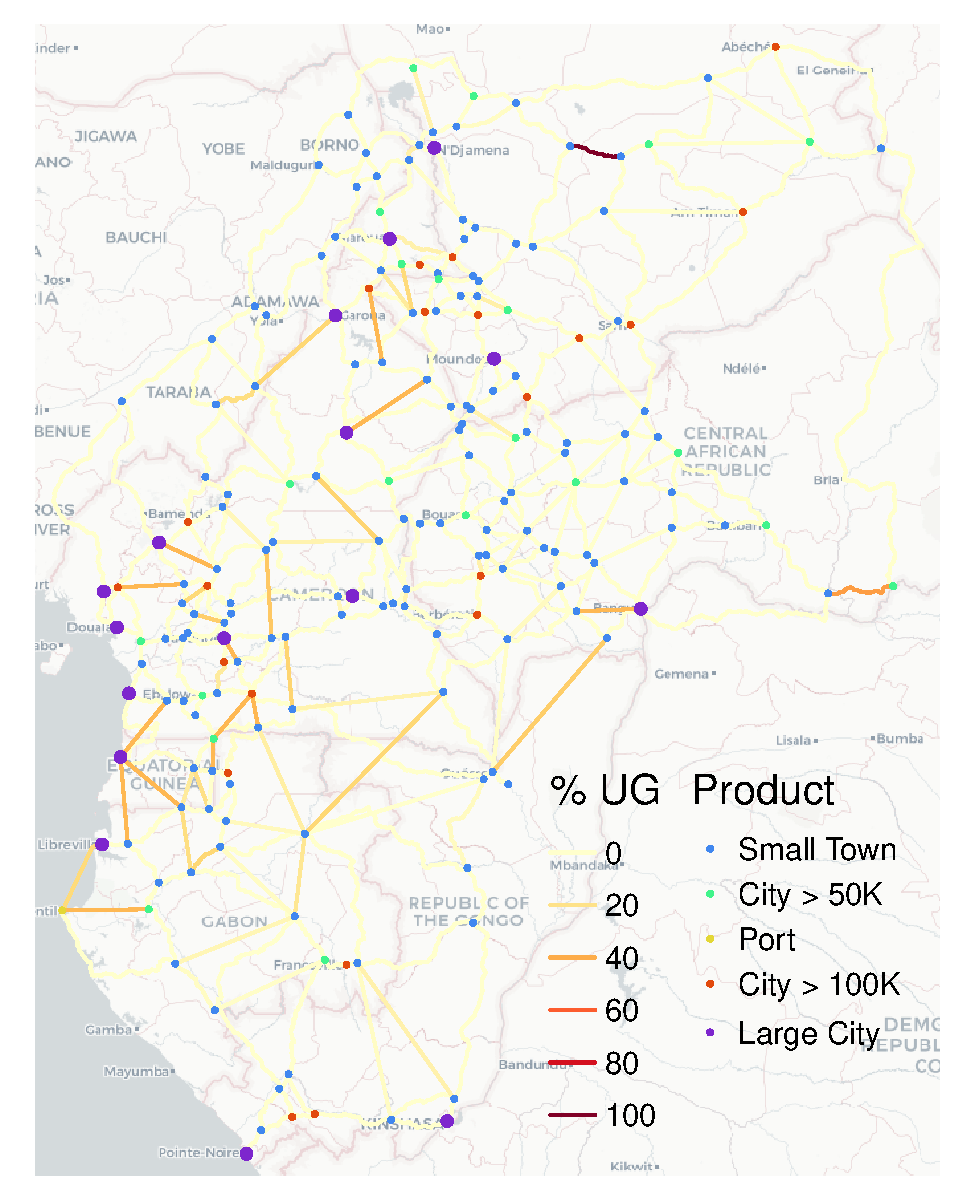
\includegraphics[width=0.38\textwidth, trim= {0.9cm 0 0.9cm 0}, clip]{"../figures/GE/trans_africa_network_GE_add_20g_1b_fixed_cgc_sigma3.8_rho0_julia_MACR_90kmh_google_perc_ug.pdf"} & 
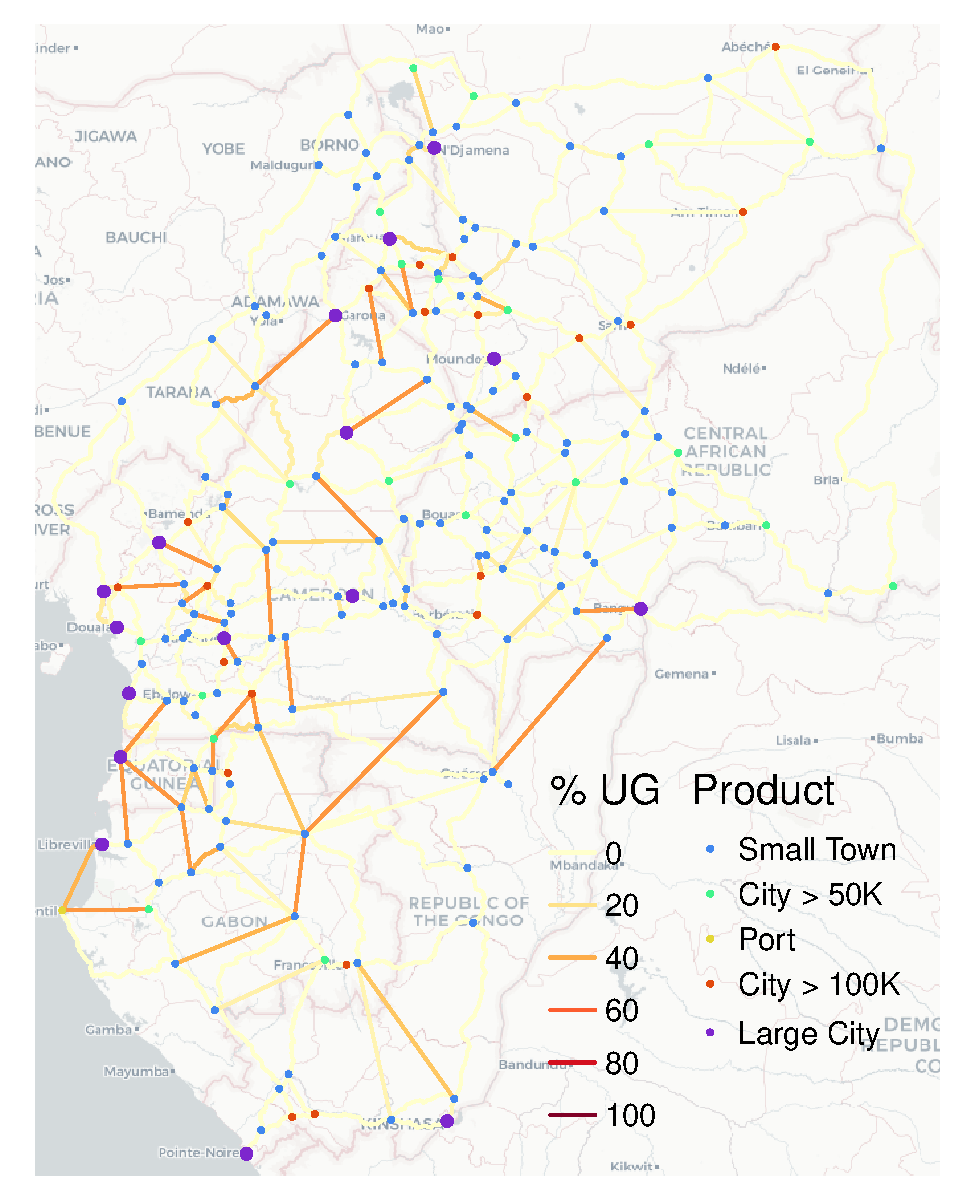
\includegraphics[width=0.38\textwidth, trim= {0.9cm 0 0.9cm 0}, clip]{"../figures/GE/trans_africa_network_GE_add_20g_2b_fixed_cgc_sigma3.8_rho0_julia_MACR_90kmh_google_perc_ug.pdf"} &
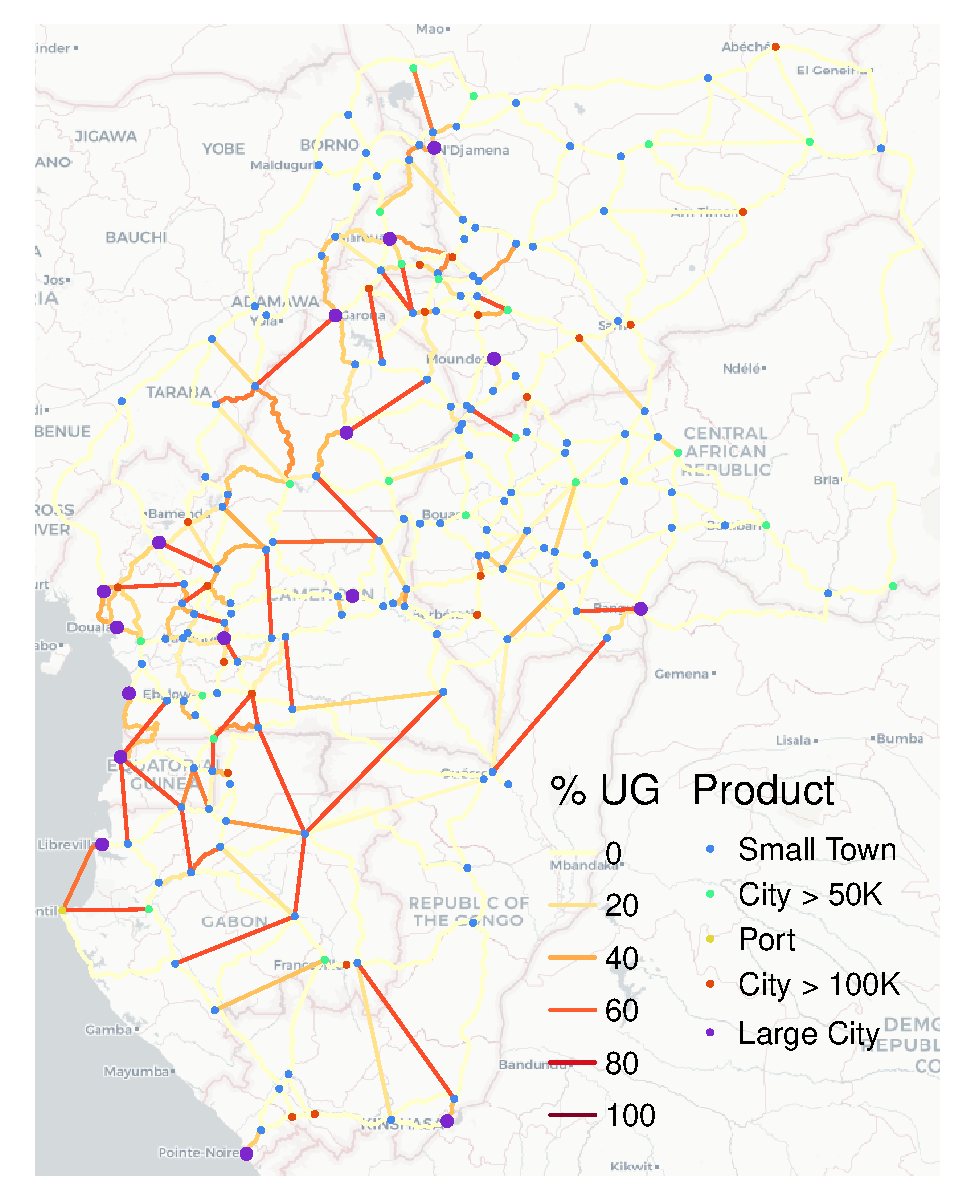
\includegraphics[width=0.38\textwidth, trim= {0.9cm 0 0.9cm 0}, clip]{"../figures/GE/trans_africa_network_GE_add_20g_4b_fixed_cgc_sigma3.8_rho0_julia_MACR_90kmh_google_perc_ug.pdf"}  
\end{tabular}
\end{adjustbox}
\end{frame}

\begin{frame}{Optimal Allocations - Inequality Aversion ($\rho = 2$)}
\vspace{-1mm}
\begin{adjustbox}{center}
\begin{tabular}{@{}c@{}|@{}c@{}|@{}c@{}} 
\$1B USD'15 & \$2B USD'15 & \$4B USD'15 \\
New: 1553km $|$ UG: 124km & New: 2878km $|$ UG: 369km & New: 5017km $|$ UG: 1529km \\ 
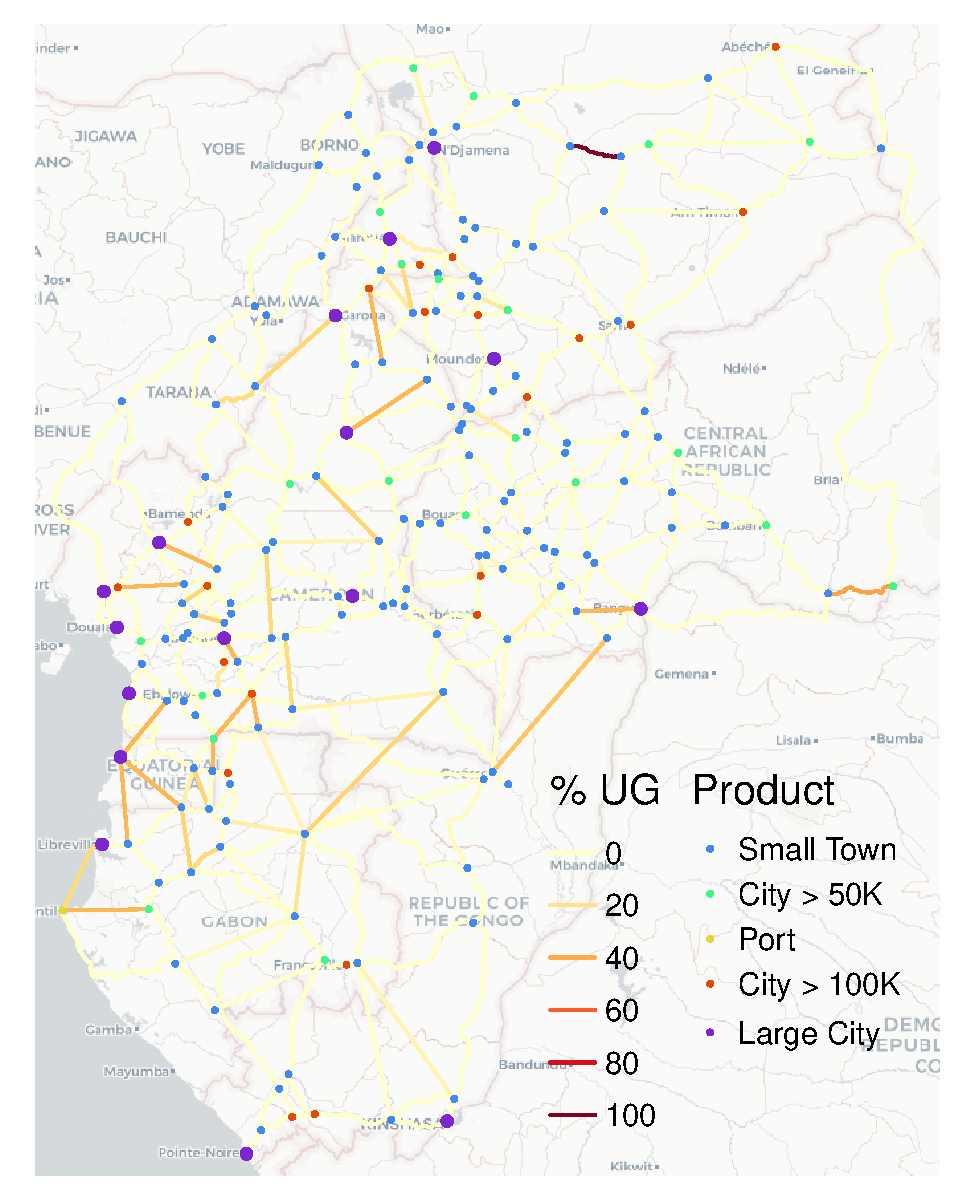
\includegraphics[width=0.38\textwidth, trim= {0.9cm 0 0.9cm 0}, clip]{"../figures/GE/trans_africa_network_GE_add_20g_1b_fixed_cgc_sigma3.8_rho2_julia_MACR_90kmh_google_perc_ug.pdf"} & 
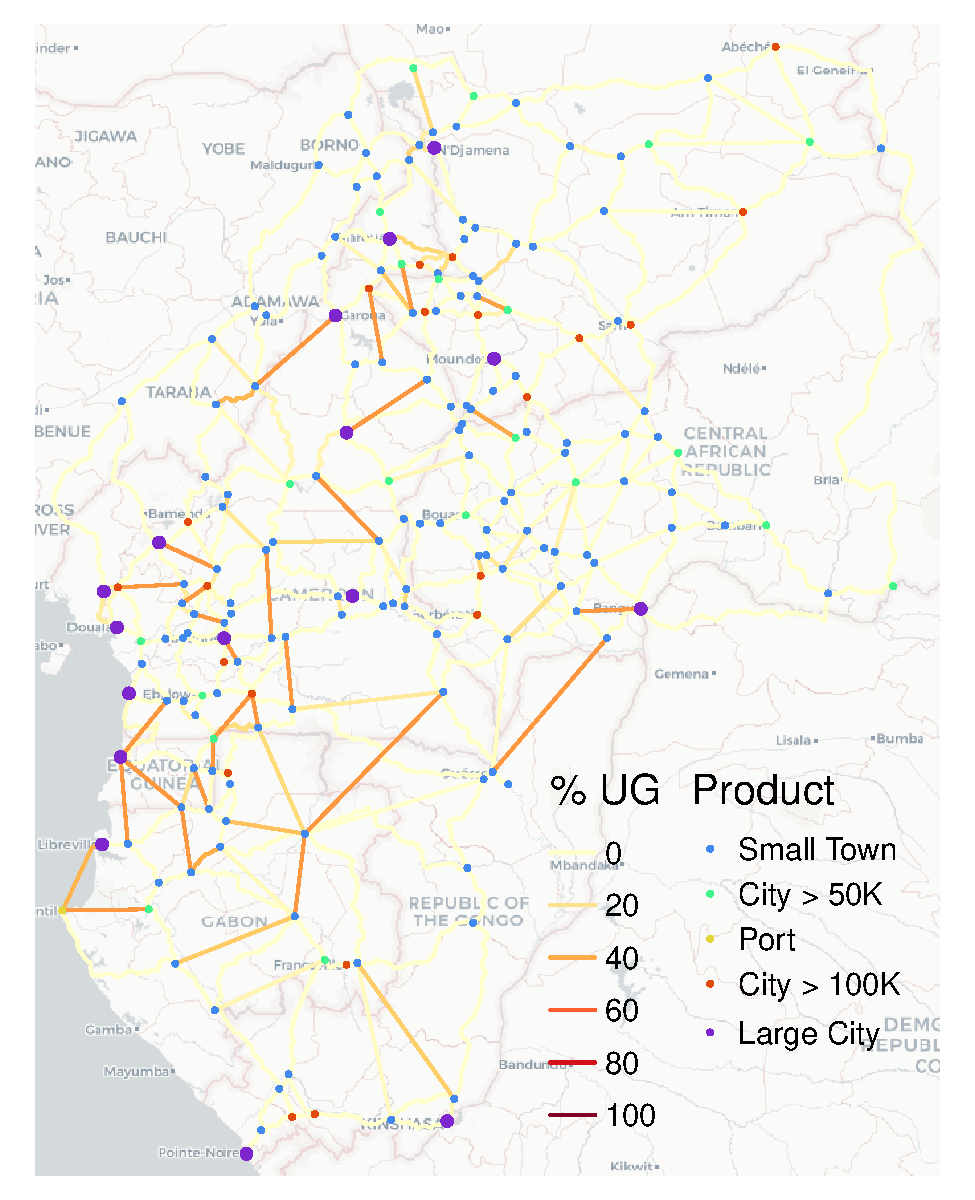
\includegraphics[width=0.38\textwidth, trim= {0.9cm 0 0.9cm 0}, clip]{"../figures/GE/trans_africa_network_GE_add_20g_2b_fixed_cgc_sigma3.8_rho2_julia_MACR_90kmh_google_perc_ug.pdf"} &
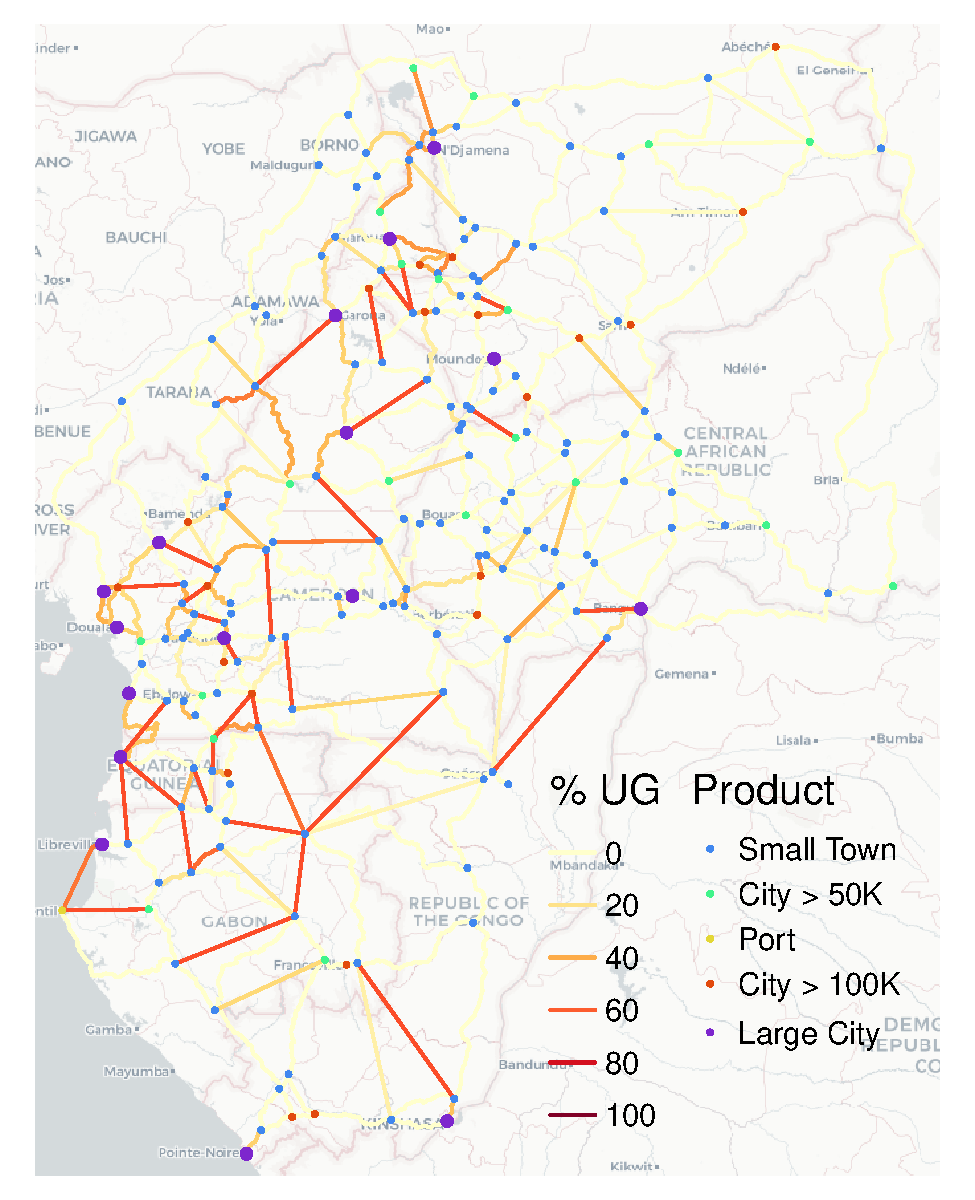
\includegraphics[width=0.38\textwidth, trim= {0.9cm 0 0.9cm 0}, clip]{"../figures/GE/trans_africa_network_GE_add_20g_4b_fixed_cgc_sigma3.8_rho2_julia_MACR_90kmh_google_perc_ug.pdf"}  
\end{tabular}
\end{adjustbox}
\end{frame}

\begin{frame}{Impact of Frictions - Only Upgrades}
\vspace{-1mm}
\begin{adjustbox}{center}
\begin{tabular}{@{}c@{}|@{}c@{}|@{}c@{}} 
\$1B USD'15 & \$2B USD'15 & \$4B USD'15 \\
Upgraded: 1543km & Upgraded: 3152km & Upgraded: 6905km \\ 
\includegraphics[width=0.38\textwidth, trim= {0.9cm 0 0.9cm 0}, clip]{"../figures/GE/trans_africa_network_GE_20g_1b_fixed_cgc_sigma3.8_rho0_julia_MACR_90kmh_google_Ijk_bc_perc_ug_diff.pdf"} & 
\includegraphics[width=0.38\textwidth, trim= {0.9cm 0 0.9cm 0}, clip]{"../figures/GE/trans_africa_network_GE_20g_2b_fixed_cgc_sigma3.8_rho0_julia_MACR_90kmh_google_Ijk_bc_perc_ug_diff.pdf"} &
\includegraphics[width=0.38\textwidth, trim= {0.9cm 0 0.9cm 0}, clip]{"../figures/GE/trans_africa_network_GE_20g_4b_fixed_cgc_sigma3.8_rho0_julia_MACR_90kmh_google_Ijk_bc_perc_ug_diff.pdf"}  
\end{tabular}
\end{adjustbox}
\end{frame}

\begin{frame}{Impact of Frictions}
\vspace{-1mm}
\begin{adjustbox}{center}
\begin{tabular}{@{}c@{}|@{}c@{}|@{}c@{}} 
\$1B USD'15 & \$2B USD'15 & \$4B USD'15 \\
New: 1607km $|$ UG: 116km & New: 2943km $|$ UG: 416km & New: 4894km $|$ UG: 1713km \\ 
\includegraphics[width=0.38\textwidth, trim= {0.9cm 0 0.9cm 0}, clip]{"../figures/GE/trans_africa_network_GE_add_20g_1b_fixed_cgc_sigma3.8_rho0_julia_MACR_90kmh_google_Ijk_bc_perc_ug_diff.pdf"} & 
\includegraphics[width=0.38\textwidth, trim= {0.9cm 0 0.9cm 0}, clip]{"../figures/GE/trans_africa_network_GE_add_20g_2b_fixed_cgc_sigma3.8_rho0_julia_MACR_90kmh_google_Ijk_bc_perc_ug_diff.pdf"} &
\includegraphics[width=0.38\textwidth, trim= {0.9cm 0 0.9cm 0}, clip]{"../figures/GE/trans_africa_network_GE_add_20g_4b_fixed_cgc_sigma3.8_rho0_julia_MACR_90kmh_google_Ijk_bc_perc_ug_diff.pdf"}  
\end{tabular}
\end{adjustbox}
\end{frame}


%------------------------------------------------
\section{Evaluating Regional Road Projects}
%------------------------------------------------

\sectionframe{Evaluating Regional Road Projects}

\begin{frame}{Regional Road Projects - MA (GDP/Minute) Gains}
\vspace{-3mm}
All road projects sum to 3.4 billion USD'15 in my calculations. They jointly yield a \textbf{28.6\%} MA gain (2.14\$/min/\$), which is larger than the sum of individual marginal gains at 23.4\%. Under frictions: \textbf{26.7\%} (1.17\$/min/\$, $\sum$ individual gains $=$ 23.2\%). \\ \vspace{-1.2mm}
\begin{adjustbox}{center}
\begin{tabular}{@{}c@{}c@{}@{}c@{}} 
\includegraphics[width=0.38\textwidth, trim= {0.9cm 0 0.9cm 0}, clip]{"../figures/PE/trans_CEMAC_network_MACR_90_min_speed_perc_planned_projects.pdf"} & 
\includegraphics[width=0.38\textwidth, trim= {0.9cm 0 0.9cm 0}, clip]{"../figures/PE/trans_CEMAC_network_MACR_90_min_speed_bt_perc_planned_projects.pdf"} & 
\includegraphics[width=0.38\textwidth, trim= {0.9cm 0 0.9cm 0}, clip]{"../figures/PE/trans_CEMAC_network_MACR_90_min_speed_bt_ratio_planned_projects.pdf"}
\end{tabular}
\end{adjustbox}
\end{frame}

\begin{frame}{Regional Road Projects - MA Returns (\$/min/\$)}
\vspace{-3mm}
All road projects sum to 3.4 billion USD'15 in my calculations. They jointly yield a \textbf{28.6\%} MA gain (2.14\$/min/\$), which is larger than the sum of individual marginal gains at 23.4\%. Under frictions: \textbf{26.7\%} (1.17\$/min/\$, $\sum$ individual gains $=$ 23.2\%). \\ \vspace{-1.2mm}
\begin{adjustbox}{center}
\begin{tabular}{@{}c@{}c@{}@{}c@{}} 
\includegraphics[width=0.38\textwidth, trim= {0.9cm 0 0.9cm 0}, clip]{"../figures/PE/trans_CEMAC_network_MACR_gain_all_90kmh_pusd_planned_projects.pdf"} & 
\includegraphics[width=0.38\textwidth, trim= {0.9cm 0 0.9cm 0}, clip]{"../figures/PE/trans_CEMAC_network_MACR_gain_all_90kmh_pusd_bt_planned_projects.pdf"} & 
\includegraphics[width=0.38\textwidth, trim= {0.9cm 0 0.9cm 0}, clip]{"../figures/PE/trans_CEMAC_network_MACR_gain_all_90kmh_pusd_bt_ratio_planned_projects.pdf"}
\end{tabular}
\end{adjustbox}
\end{frame}

\begin{frame}{Regional Road Projects - Optimal GE Allocation of \$3.4B USD'15}
\vspace{-1mm}
\begin{adjustbox}{center}
\begin{tabular}{@{}c@{}|@{}c@{}|@{}c@{}} 
Upgrades & Upgrades Ineq. Av. & New Links + Upgrades \\
Upgraded: 5350km & Upgraded: 5128km & New: 4213km $|$ UG: 1154km \\ 
\includegraphics[width=0.38\textwidth, trim= {0.9cm 0 0.9cm 0}, clip]{"../figures/GE/trans_africa_network_GE_20g_3200m_fixed_cgc_sigma3.8_rho0_julia_MACR_90kmh_google_perc_ug.pdf"} & 
\includegraphics[width=0.38\textwidth, trim= {0.9cm 0 0.9cm 0}, clip]{"../figures/GE/trans_africa_network_GE_20g_3200m_fixed_cgc_sigma3.8_rho2_julia_MACR_90kmh_google_perc_ug.pdf"} &
\includegraphics[width=0.38\textwidth, trim= {0.9cm 0 0.9cm 0}, clip]{"../figures/GE/trans_africa_network_GE_add_20g_3200m_fixed_cgc_sigma3.8_rho0_julia_MACR_90kmh_google_perc_ug.pdf"}  
\end{tabular}
\end{adjustbox}
\end{frame}

%------------------------------------------------
\section{Conclusions}
%------------------------------------------------

\begin{frame}{Conclusions}
  \begin{itemize} 
  	\item Road investments in Cameroon (Douala-Yaounde and up north toward N'Djamena) and in borders crossing to Cameroon yield greatest marginal benefits (Cameroon $=$ 46\% of CEMAC GDP and 45\% of CEMAC population).
  	\item 100\% border frictions reduction yields 58\% MA gain, vs. 64\% gain from upgrades to 90km/h (\$19B USD'15) and 72\% from upgrades + \$8B USD'15 new links. 
  	\item \$4B-\$5B USD'15 high-yield-links road packages (or below) can yield 43\%-53\% MA gains and should be highly-profitable in medium run (30-year PDV profitability requires 1\% increase in macroeconomic growth rate at 3.5\% baseline growth). 
  	\item Planned works estimated at \$3.4B USD'15 yield 27-29\% MA gain (1.2-2.1\$/min/\$ vs. 1.4-2.8\$/min/\$ for the \$4B-\$5B PE packages) $\to$ modest inefficiency.
    \item GE planners invest more in new links than upgrades if given the choice - unlike Africa \citep{krantz2024optimal} $\to$ strong indication that network needs to be expanded. (Also: inequality averse planners invest more in poorer north (Chad, CAR)).
  \end{itemize}
\end{frame}

% Set total frame count before appendix
\setcounter{totalframecount}{\value{framenumber}}

% Thank you slide
\begin{frame}[plain]
  \centering
    \vspace{0.8cm}
   \huge{\color{RoyalBlue}Thank you!}
   
  \vspace{0.5cm}
  
  \large{Sebastian Krantz}\\
  \small{Kiel Institute for the World Economy}\\
  \small{\texttt{sebastian.krantz@ifw-kiel.de}}\\ \vspace{1em}
  \small{Paper $+$ Slides Available at}\\
  \small{\href{https://sebastiankrantz.com}{\texttt{sebastiankrantz.com}}}\\ \vspace{1em}
  \small{Replication Package $+$ Transport Network Optimization Libraries}\\
  \small{\href{https://github.com/SebKrantz/OptimalTransportNetworks}{\texttt{github.com/SebKrantz/OptimalTransportNetworks}}}\\
  \vspace{0.3cm}
  % \includegraphics[width = 0.35\textwidth]{"../figures/IfW_Logo_master_en.png"}
\end{frame}

\setcounter{framenumber}{0}
\renewcommand{\insertframenumber}{R\arabic{framenumber}}

\begin{frame}{References}
\bibliographystyle{apacite}
\bibliography{bibliography}  % This links to a file bibliography.bib with the citations
\end{frame}

%------------------------------------------------
% Appendix 
%------------------------------------------------

\appendix
% Start of your appendix
\setcounter{framenumber}{0}
\renewcommand{\insertframenumber}{A\arabic{framenumber}}
\setcounter{table}{0}
\renewcommand{\thetable}{A\arabic{table}}
\setcounter{figure}{0}
\renewcommand{\thefigure}{A\arabic{figure}}

\begin{frame}[label=GEModelSol]{Optimal Transport Networks in Spatial Equilibrium \quad \hyperlink{GEModel}{\beamergotobutton{back}}}
$\exists$ (more complex) model variants with cross-goods congestion and mobile labor. I assume cross-goods congestion but keep labour fixed (due to trade through ports).  \\ \vspace{4mm}

Equilibrium prices $P^n_j$ are the Lagrange multipliers on the flows constraints (Eq. \ref{eq:BALFL}), and $P_K$ is the multiplier on the network building constraint (shadow price of asphalt). Then 
\begin{equation}
I^*_{jk} = \left[ \frac{\gamma}{P_K \delta^I_{jk} (\delta^\tau_{jk})^{\frac{1}{\beta}}} \left( \frac{1}{1+\beta} \sum_{n: P^n_k > P^n_j} P^n_j \left( \frac{P^n_k}{P^n_j} - 1 \right)^{\frac{1+\beta}{\beta}} \right) \right]^{\frac{\beta}{\beta-\gamma}}.
\end{equation}
Planners problem is only convex if $\beta \geq \gamma$, i.e., if congestion forces are stronger than returns to infrastructure (DRS). But \citet{fajgelbaum2020optimal} also approximate the non-convex case ($\beta < \gamma \to$ IRS in infrastructure) using simulated annealing methods. \\\vspace{2mm}
\begin{itemize}
\item Optimal road investments directed to locations with initially lower levels ($I^0_{jk}$), higher population ($L_j$), and productivity ($Z_j^n$ $\sim$ income per worker). 
\item IRS incentivizes planner to concentrate flows on a few links (tree-like network).
\end{itemize}
\end{frame}

\begin{frame}[label=EXPOU]{Exports - Only Upgrades \quad \hyperlink{IOU}{\beamergotobutton{back}}}
\begin{tabular}{cc} 
\$1B: & \includegraphics[width=0.9\textwidth, trim= {0 5mm 0 5mm}, clip]{"../figures/GE/trans_africa_network_GE_20g_1b_fixed_cgc_sigma3.8_rho0_julia_MACR_90kmh_google_good_flows_4_city.pdf"} \\
\$4B: & \includegraphics[width=0.9\textwidth, trim= {0 5mm 0 5mm}, clip]{"../figures/GE/trans_africa_network_GE_20g_4b_fixed_cgc_sigma3.8_rho0_julia_MACR_90kmh_google_good_flows_4_city.pdf"}  
\end{tabular}
\end{frame}

\begin{frame}[label=EXP]{Exports \quad \hyperlink{III}{\beamergotobutton{back}}}
\begin{tabular}{cc} 
\$1B: & \includegraphics[width=0.9\textwidth, trim= {0 5mm 0 5mm}, clip]{"../figures/GE/trans_africa_network_GE_add_20g_1b_fixed_cgc_sigma3.8_rho0_julia_MACR_90kmh_google_good_flows_4_city.pdf"} \\
\$4B: & \includegraphics[width=0.9\textwidth, trim= {0 5mm 0 5mm}, clip]{"../figures/GE/trans_africa_network_GE_add_20g_4b_fixed_cgc_sigma3.8_rho0_julia_MACR_90kmh_google_good_flows_4_city.pdf"}  
\end{tabular}
\end{frame}


\end{document}